% Copyright 2023 Fausto Spoto
%
% Licensed under the Apache License, Version 2.0 (the "License");
% you may not use this file except in compliance with the License.
% You may obtain a copy of the License at
%
%    http://www.apache.org/licenses/LICENSE-2.0
%
% Unless required by applicable law or agreed to in writing, software
% distributed under the License is distributed on an "AS IS" BASIS,
% WITHOUT WARRANTIES OR CONDITIONS OF ANY KIND, either express or implied.
% See the License for the specific language governing permissions and
% limitations under the License.

\documentclass[11pt]{beamer}  %% versione proiettore
%%\documentclass[11pt,handout]{beamer} %% versione stampa
\usepackage{lucidiJb-2ed}

\usepackage{mathtools}
\usepackage{relsize}

\mode<article>
{
  \usepackage{fullpage}
  \usepackage{hyperref}
}

\mode<presentation>
{
  \setbeamertemplate{background canvas}[vertical shading][bottom=red!10,top=blue!10]
  \usetheme{Course}
  \usefonttheme[onlysmall]{structurebold}
}

\subtitle{R\'eunion Island, 13/4/2023}
\title{An Overview of Blockchain Technology}
\institute{Universit\`a di Verona, Italy}
\date{April 2023}

\setbeamercovered{invisible}

\def\codesize{\smaller}
\def\<#1>{\codeid{#1}}
\newcommand{\codeid}[1]{\ifmmode{\mbox{\codesize\ttfamily{#1}}}\else{\codesize\ttfamily #1}\fi}

\AtBeginSection[]{
  \begin{frame}
  \vfill
  \centering
  \begin{beamercolorbox}[sep=8pt,center,shadow=true,rounded=true]{title}
    \usebeamerfont{title}\insertsectionhead\par%
  \end{beamercolorbox}
  \vfill
  \end{frame}
}

\begin{document}

\begin{frame}
  \titlepage
\end{frame}

\begin{frame}
  \tableofcontents
\end{frame}

\section{Introduction}

\begin{frame}\frametitle{The mainstream view of blockchain}

  \begin{center}
    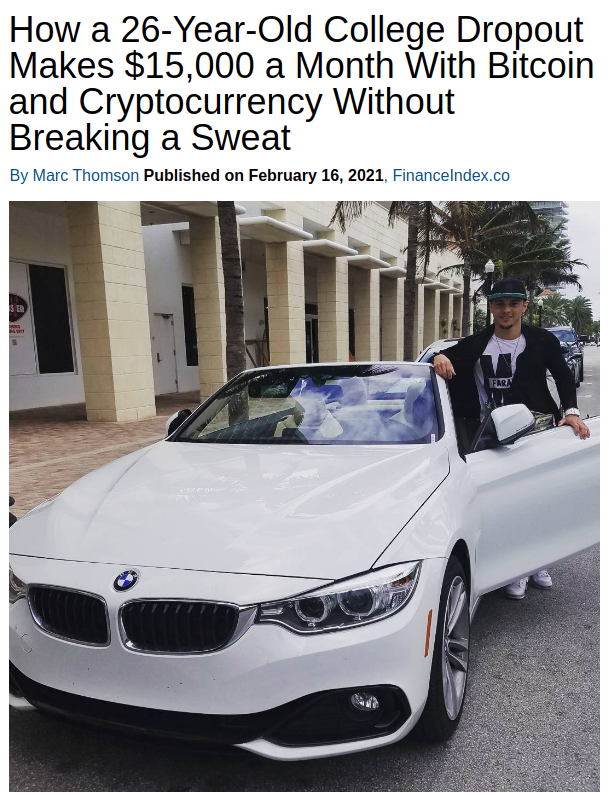
\includegraphics[scale=0.209,clip=false]{pictures/dropout.png}
    \hspace*{2ex}
    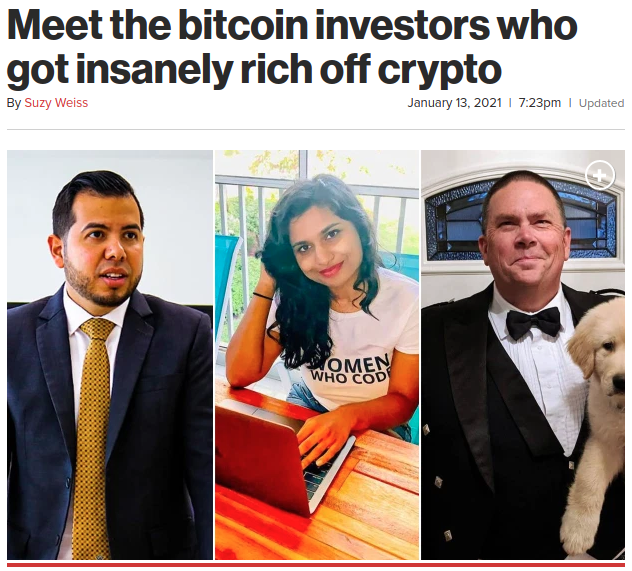
\includegraphics[scale=0.29,clip=false]{pictures/insane.png}
  \end{center}

\end{frame}

\begin{frame}\frametitle{History}

  \begin{itemize}
  \item[1988] proof-of-work (Dwork \& Naor)
  \item[1991] a cryptographically secure chain of blocks (Haber \& Stornetta)
  \item[199x] smart contracts (Szabo)
  \item[2008] Bitcoin (Nakamoto)
  \item[2012] proof-of-stake (Peercoin)
  \item[2013] Ethereum (Buterin \& Wood)
  \item[2014] proof-of-space (Burstcoin/Signum)
  \item[2014] Tendermint generic proof-of-stake engine (Kwon)
  \item[2022] Ethereum 2.0 adopts the proof-of-stake
  \end{itemize}
  
\end{frame}

\begin{frame}\frametitle{Distributed network}

  \begin{center}
    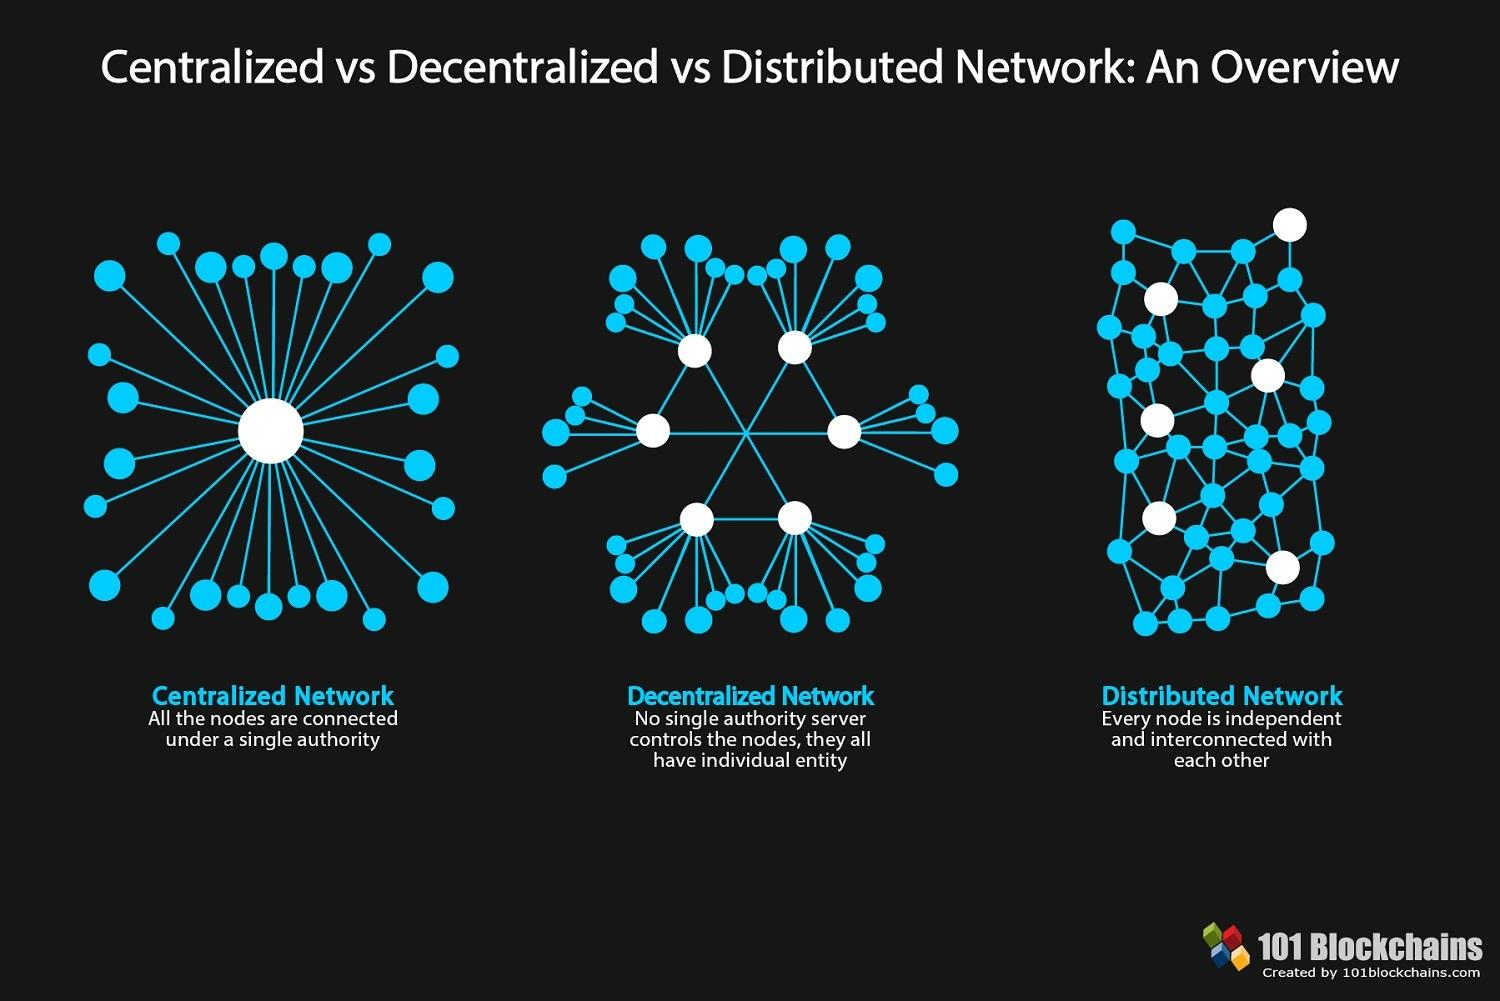
\includegraphics[scale=0.22,clip=false]{pictures/distributed.jpg}
  \end{center}

\end{frame}

\begin{frame}\frametitle{Cryptocurrencies}

  \begin{center}
    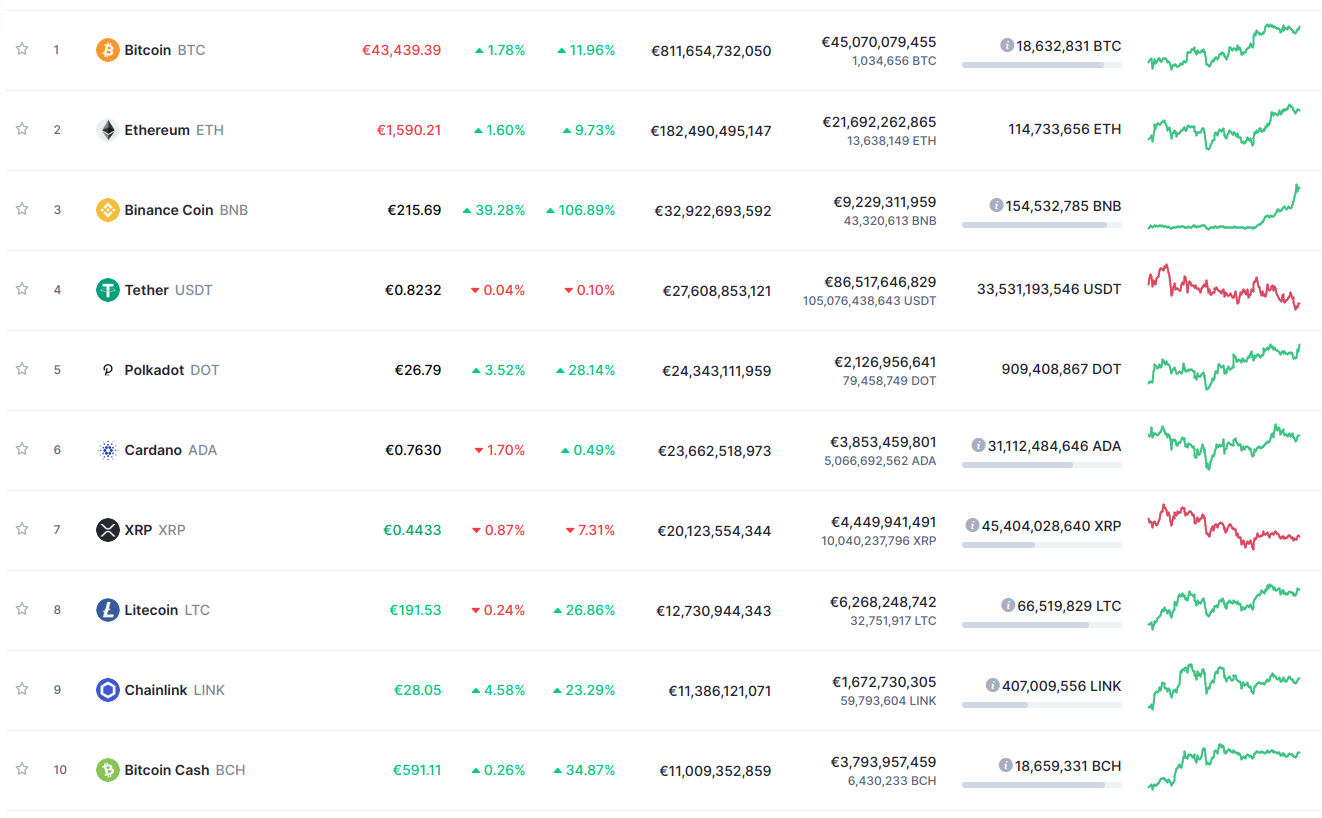
\includegraphics[scale=0.258,clip=false]{pictures/market.png}
  \end{center}

\end{frame}

\begin{frame}\frametitle{Bitcoin chart}

  \begin{center}
    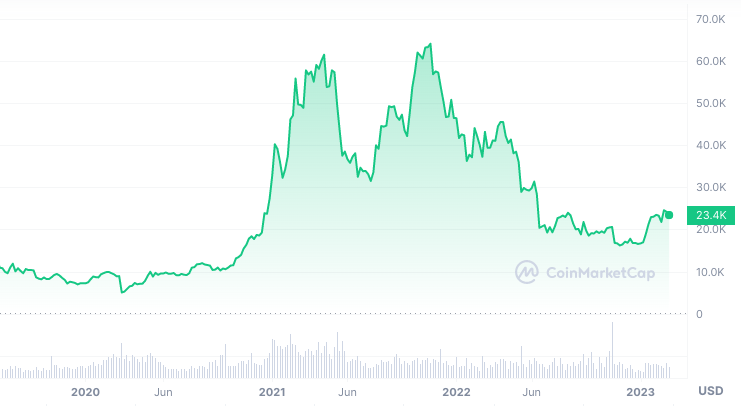
\includegraphics[width=\textwidth,clip=false]{pictures/bitcoin-coinmarketcap.png}
  \end{center}

\end{frame}

\begin{frame}\frametitle{Bitcoin capitalization (2018)}

  \begin{center}
    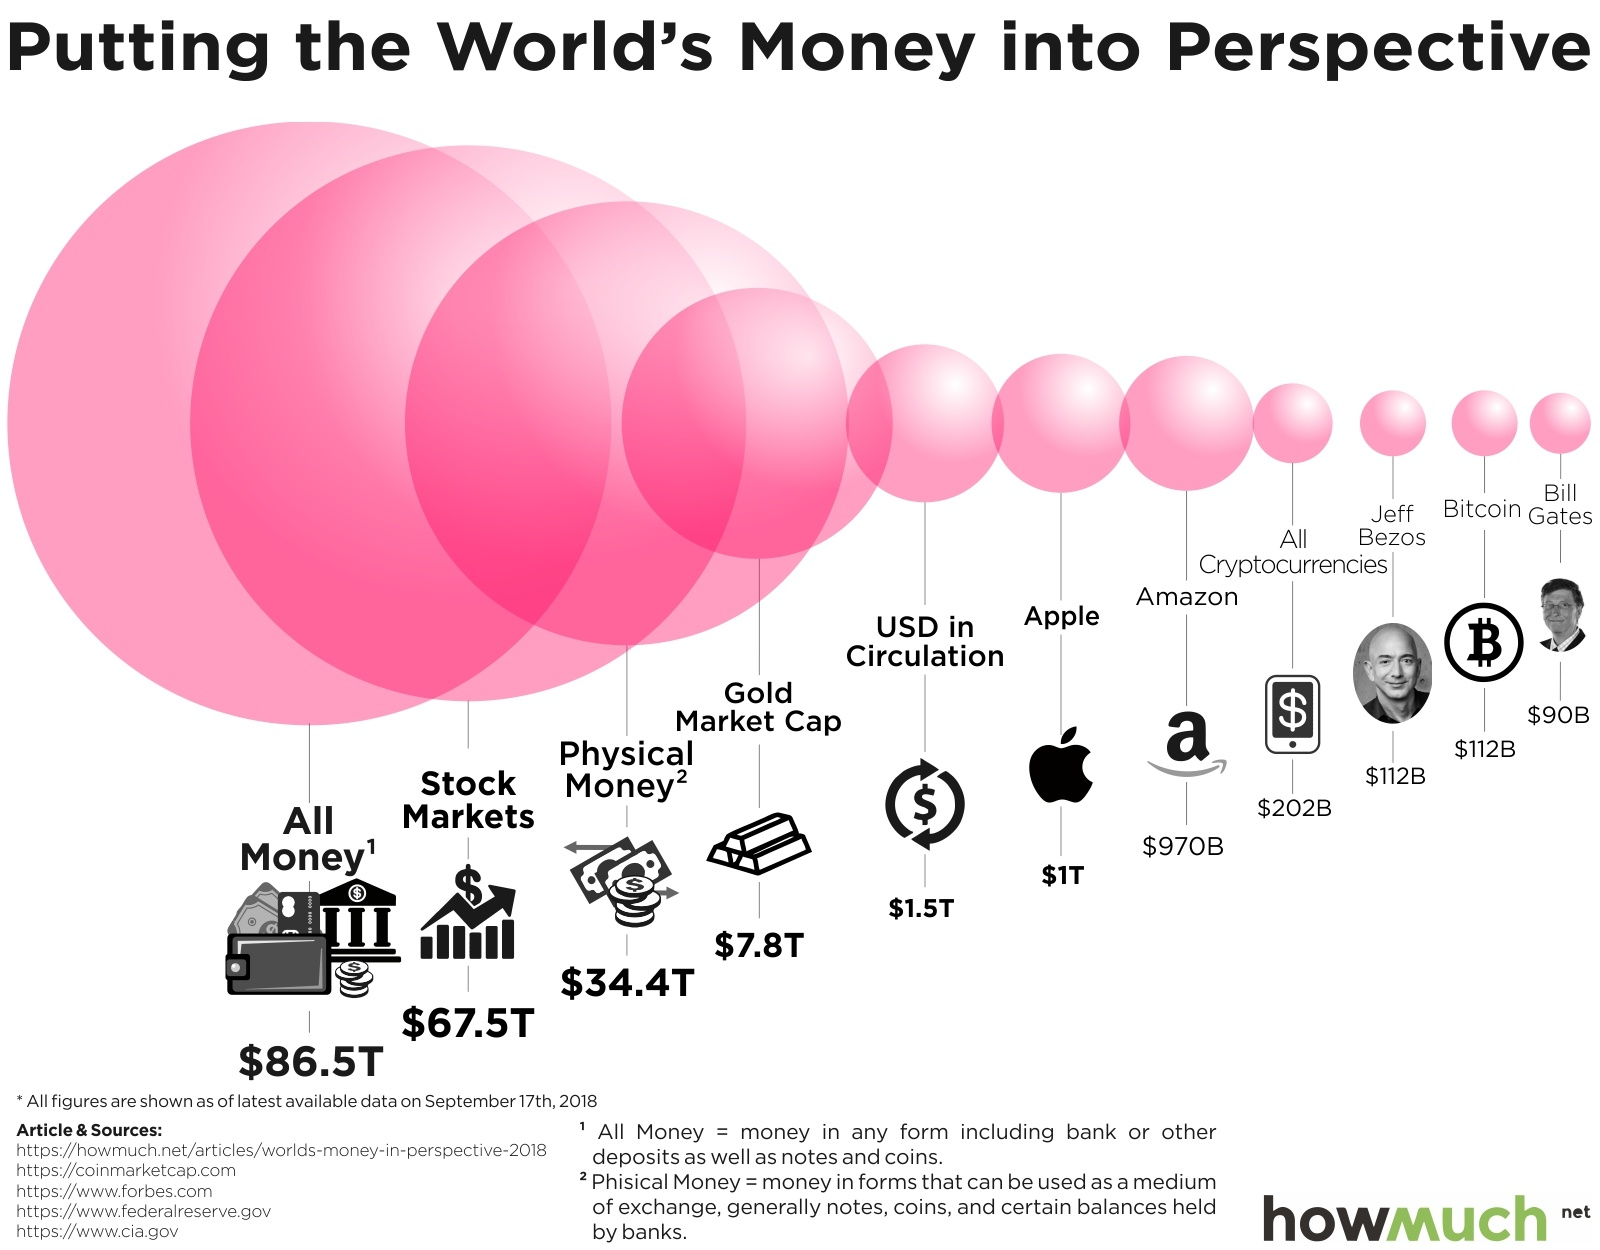
\includegraphics[scale=0.16,clip=false]{pictures/bitcoin-capitalization.jpg}
  \end{center}

  \begin{center}
    source: \url{HowMuch.net}, a financial literacy website
  \end{center}

\end{frame}

\begin{frame}\frametitle{Bitcoin transactions}

  \begin{center}
    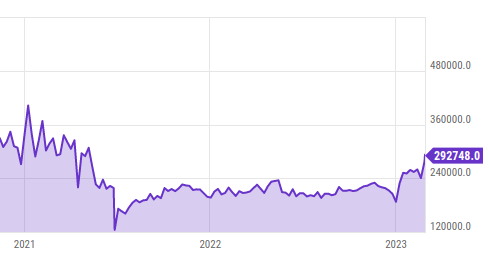
\includegraphics[scale=0.7,clip=false]{pictures/bitcoin-daily.png}
  \end{center}

  \begin{center}
    Around 300,000 transactions per day
  \end{center}

\end{frame}

\begin{frame}\frametitle{Credit cards transactions (billions, 2018)}

  \begin{center}
    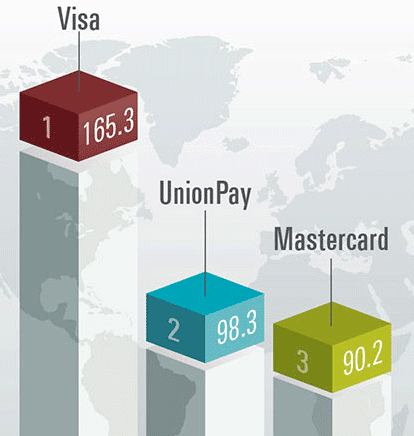
\includegraphics[scale=0.3,clip=false]{pictures/credit-cards.png}
  \end{center}

  \begin{center}
    Visa: around 451,639,000 transactions per day\\
    UnionPay: around 268,579,000 transactions per day\\
    Mastercard: around 246,448,000 transactions per day\\
    Bitcoin: around 300,000 transactions per day
  \end{center}

\end{frame}

\begin{frame}\frametitle{Bitcoin transaction fees}

  \begin{center}
    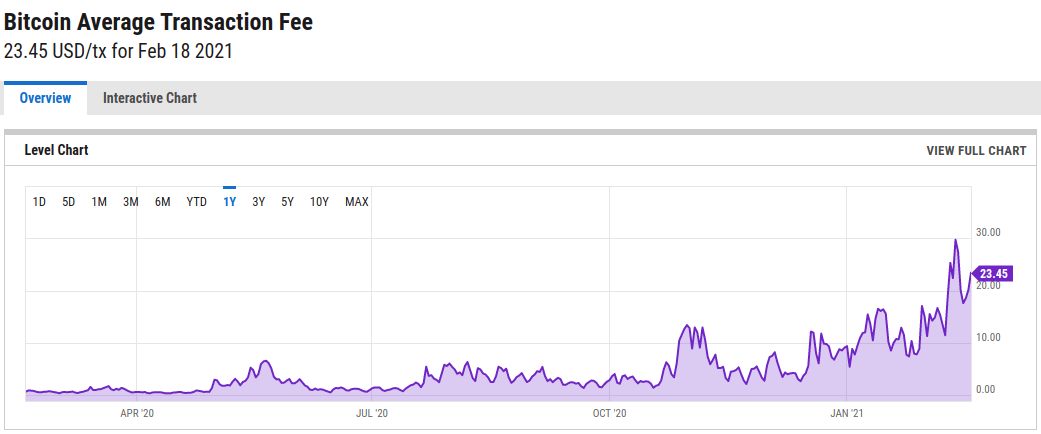
\includegraphics[width=\textwidth,clip=false]{pictures/bitcoin-fees.png}
  \end{center}

  \begin{center}
    Independent from the transacted value
  \end{center}

\end{frame}

\begin{frame}\frametitle{Credit cards transaction fees}

  \begin{center}
    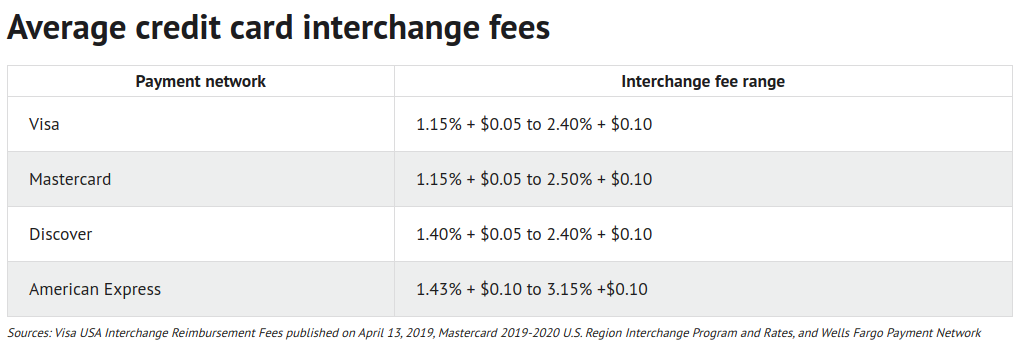
\includegraphics[width=\textwidth,clip=false]{pictures/credit-cards-fees.png}
  \end{center}

  \begin{center}
    Proportional to the transacted value
  \end{center}

\end{frame}

\begin{frame}\frametitle{The hype cycle}

  \begin{center}
    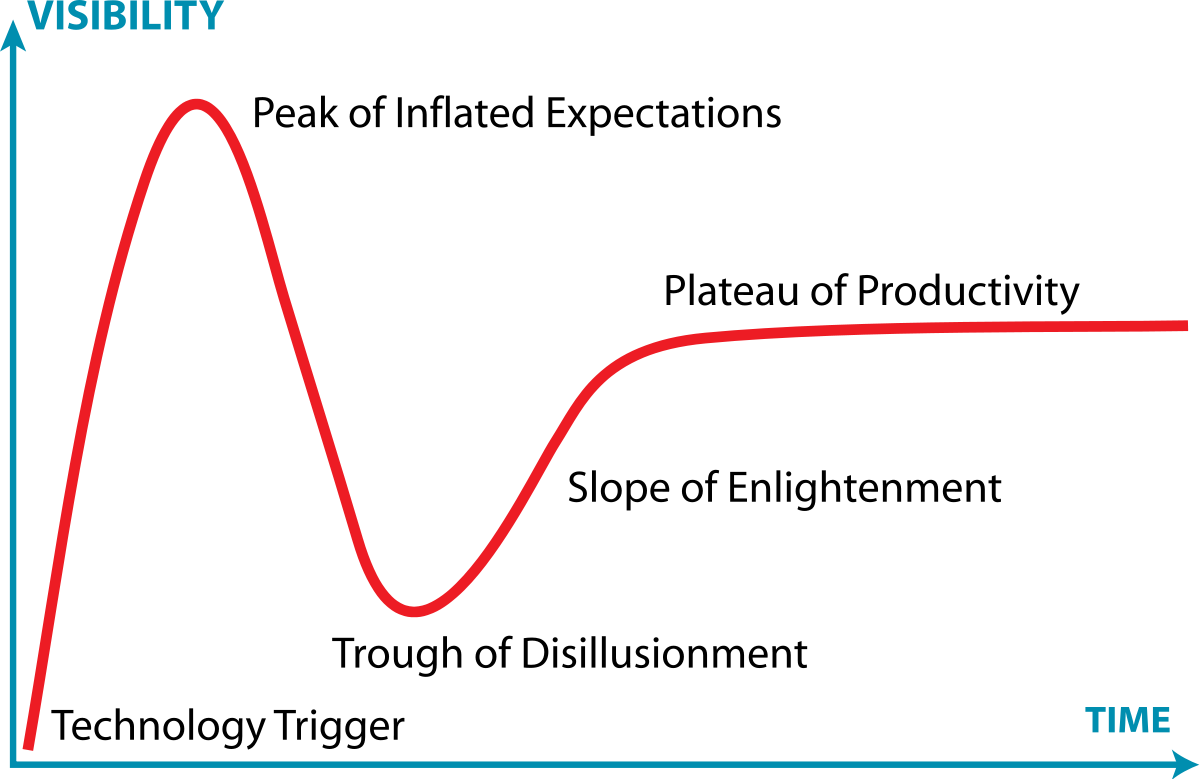
\includegraphics[width=\textwidth,clip=false]{pictures/hype-cycle.png}
  \end{center}

\end{frame}

\begin{frame}\frametitle{Beyond the hype}

  \begin{center}
    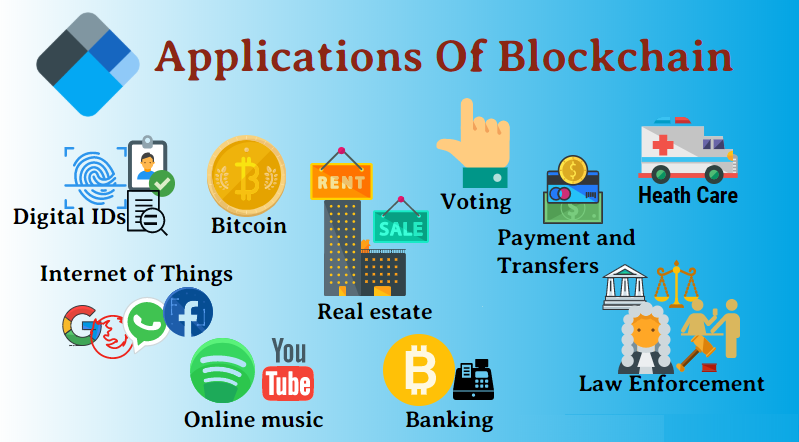
\includegraphics[scale=0.4,clip=false]{pictures/blockchain-applications.png}
  \end{center}

\end{frame}

\begin{frame}\frametitle{Future trends}

  \begin{itemize}
  \item \alert{\url{https://ipfs.io}}: decentralized file storage
  \item \alert{\url{https://identity.foundation}}: decentralized identity
  \item \alert{\url{https://defipulse.com}}: decentralized finance (DeFi)
  \item \alert{\url{https://pkt.cash}}: decentralized internet service providers
  \item integration with the internet of things
  \end{itemize}

  \begin{center}
    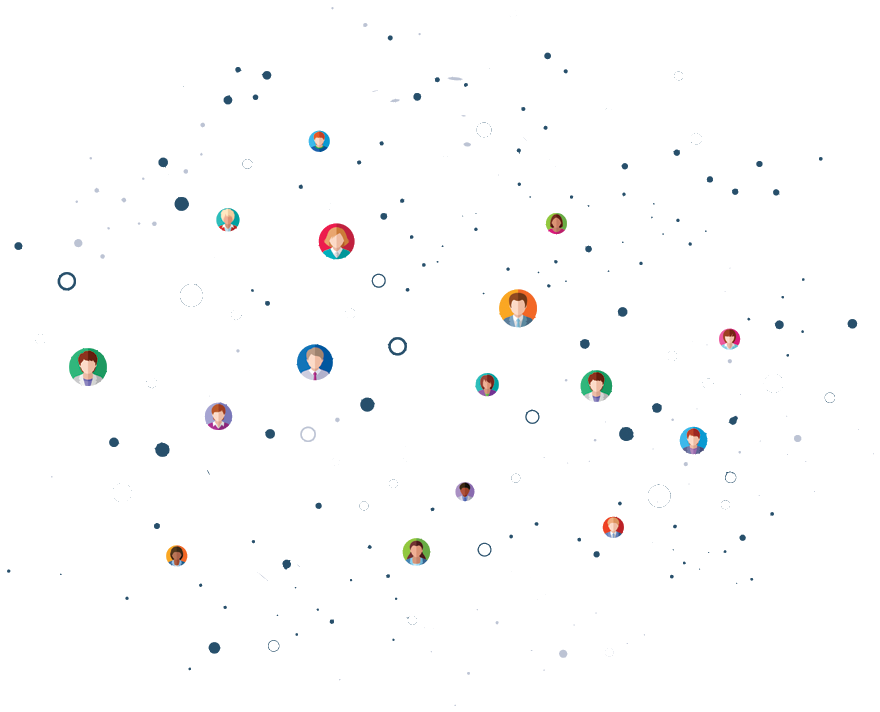
\includegraphics[scale=0.16,clip=false]{pictures/did.png}
  \end{center}

\end{frame}

\section{Bitcoin (proof of work)}

\begin{frame}
  \frametitle{The internet of money}

  \begin{greenbox}{What we expect from money}
    \begin{itemize}
    \item money should be protected from counterfeiting (\emph{legality})
    \item money should not be spent twice (\emph{uniqueness})
    \item no one can claim that my money belongs to him (\emph{ownership})
    \item money should be untained (\emph{fungibility})
    \item money should be movable (\emph{liquidity})
    \end{itemize}
  \end{greenbox}

  \bigskip

  Electronic money exists since decades (credit cards, online transactions)

  \bigskip

  \begin{greenbox}{}
    Bitcoin provides a \alert{fully decentralized} electronic cash system, for the first time
    (a single State cannot shut down the bitcoin network)
  \end{greenbox}

  \bigskip

  ``Bitcoin: A Peer-to-Peer Electronic Cash System'' by Satoshi Nakamoto, 2008

\end{frame}

\begin{frame}\frametitle{The best reference}

  \begin{center}
    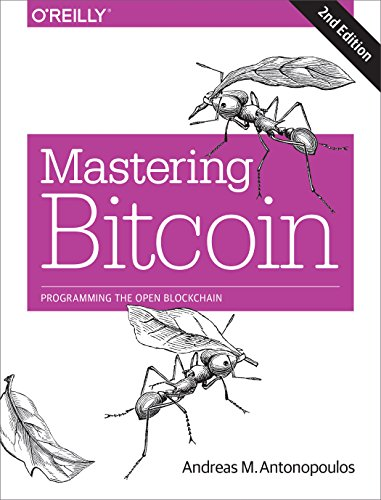
\includegraphics[scale=.35,clip=false]{pictures/mastering-bitcoin.jpg}
  \end{center}

  \begin{center}
    \url{https://github.com/bitcoinbook/bitcoinbook}
  \end{center}

\end{frame}

\begin{frame}\frametitle{Bitcoin as a web service}

  \begin{center}
    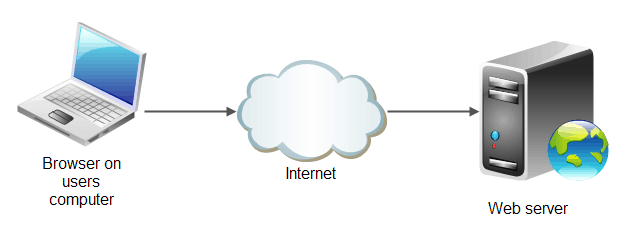
\includegraphics[scale=.3,clip=false]{pictures/web-server.png}
  \end{center}

  \medskip

  The server keeps a map (\alert{ledger}) $\mathit{user\_id}\Rightarrow\mathit{balance}$
  and accepts transactions to transfer balances

  \medskip

  Users interact through a browser (\alert{wallet}) to ask to transfer balances

  \medskip
  The server is actually a worldwide peer-to-peer (p2p) network of computers

  \begin{center}
    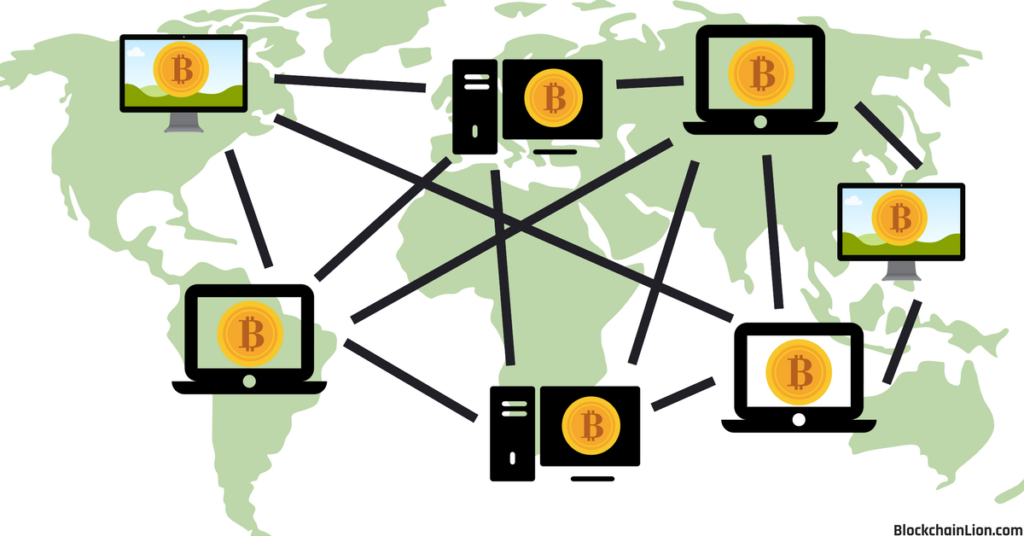
\includegraphics[scale=.13,clip=false]{pictures/distributed.png}
  \end{center}

\end{frame}

\begin{frame}\frametitle{Mobile wallets}

  At the first start-up, a bitcoin address is created for you, then transactions
  from/to that address are tracked:

  \begin{center}
    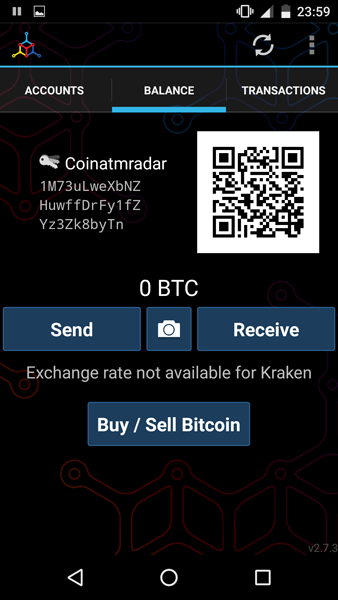
\includegraphics[scale=0.27,clip=false]{pictures/bitcoin-wallet.png}
  \end{center}

  The \alert{address} can be seen as our IBAN. Its creation
  is a local operation that does not do anything on the network: fully anonymous

\end{frame}

\begin{frame}\frametitle{Address creation}

  When Alice's wallet starts for the first time:

  \begin{enumerate}
  \item it generates a finite sequence of bits through a secure random generator
    (a secret private key)
  \item it computes the bitcoin address as an abstraction of the private key
    (hashing)
  \item it shows the bitcoin address as an alphanumeric string and as a picture (QR code)
  \item \alert{the address is not sensitive information}: Alice can publish it in her web page
  \item \alert{the private key is sensitive information}: Alice keeps it secret
    \begin{itemize}
    \item a hardware wallet stores it in its internal memory
    \item a desktop wallet stores it in Alice's computer's file system (!)
    \item a mobile wallet stores it in Alice's phone (!!!)
    \item a web wallet stores it at a third-party service (!!!!!!!)
    \end{itemize}
  \end{enumerate}
\end{frame}

\begin{frame}\frametitle{Alice charges her wallet}
  \begin{itemize}
  \item she asks a friend to send bitcoins at her address
  \item meets a bitcoin seller in person
  \item earns bitcoin by working
  \item uses a bitcoin ATM
  \item uses a bitcoin currency exchange company
  \end{itemize}

  \bigskip

  \begin{greenbox}{What is the price?}
    It is not set by the computer network! It's a social
    agreement, the average of the last sell operations.
    You can look online for it
  \end{greenbox}

\end{frame}

\begin{frame}\frametitle{The charge transaction}

  \begin{enumerate}
  \item Joe (the seller) specifies in his wallet Alice's bitcoin address
    as destination (or scans Alice's QR code with his mobile)
  \item Joe signs a transaction (a sequence of bits),
    with his private key, stating: \emph{``I acknowledge
    to send X bitcoins from my address to Alice's destination address''}
  \item Joe's wallet broadcasts the signed transactions
    to one (or more) servers of the bitcoin network
  \item the network spreads the information and eventually the transaction is cleared
    (in $10$ minutes or more)
  \item Alice's wallet polls the bitcoin network for a transaction having
    Alice's address as destination and updates the balance on the screen
    accordingly (\alert{confirmation})
  \end{enumerate}

\end{frame}

\begin{frame}\frametitle{The spend transaction}

  Alice's wallet is charged now and she wants to buy a coffee at Bob's coffee shop:

  \begin{enumerate}
  \item Alice's wallet signs, with her private key, a transaction
    (a sequence of bits) stating: \emph{``I acknowledge to send Y bitcoins from Alice's address
    to Bob's destination address''} (some metadata can be added)
  \item the transaction is broadcast to one (or more) nodes of the
    bitcoin network and eventually cleared
  \item Alice's wallet polls the bitcoin network for a transaction having
    her address as source and updates the balance on the screen
    accordingly (\alert{confirmation})
  \end{enumerate}

  \medskip
  See it online:
  {\scriptsize\url{https://explorer.btc.com/btc/transaction/0627052b6f28912f2703066a912ea577f2ce4da4caa5a5fbd8a57286c345c2f2}}

\end{frame}

\begin{frame}\frametitle{The transaction}

  \begin{center}
    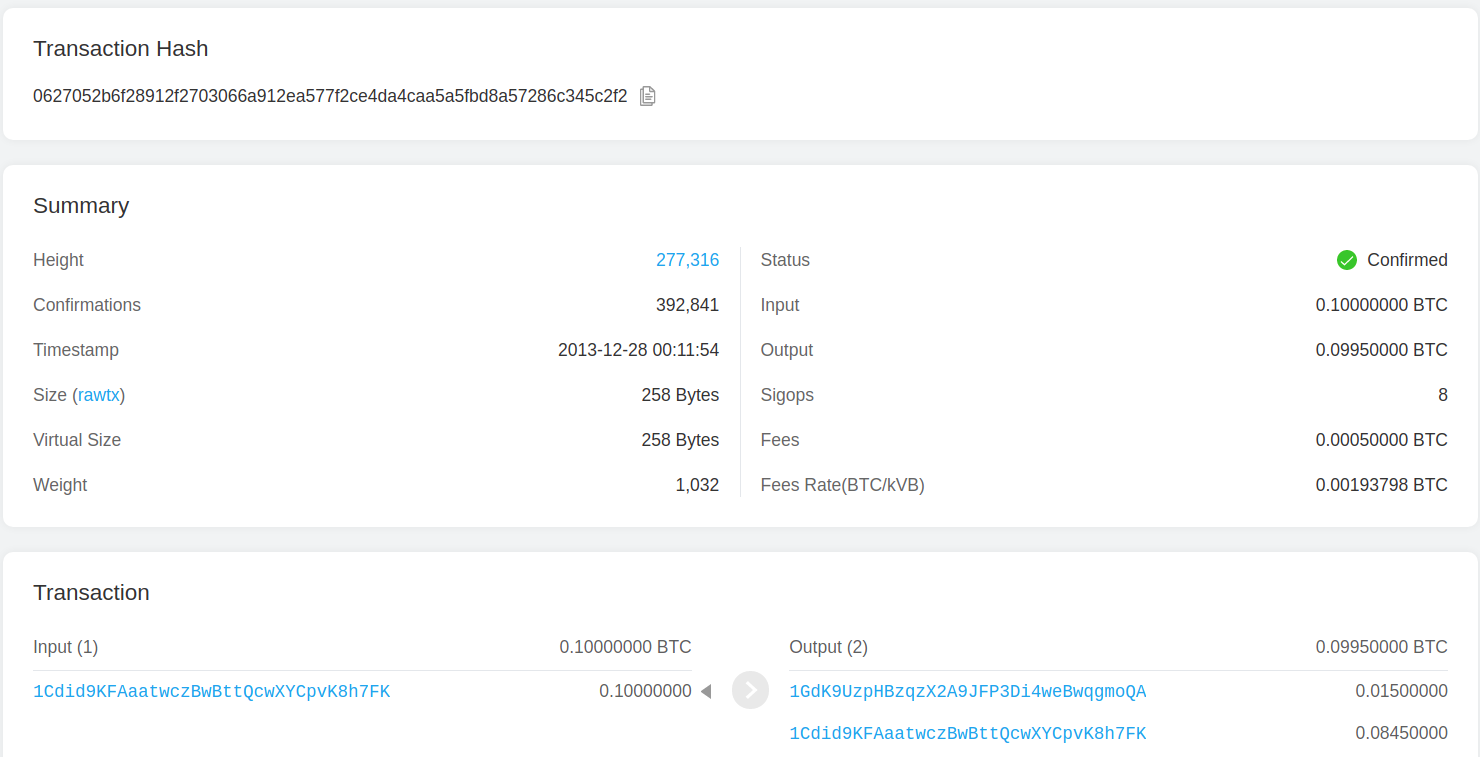
\includegraphics[scale=0.23,clip=false]{pictures/bitcoin-spend.png}
  \end{center}

\end{frame}

\begin{frame}\frametitle{Transactions form a chain, outputs can be change}

  \begin{center}
    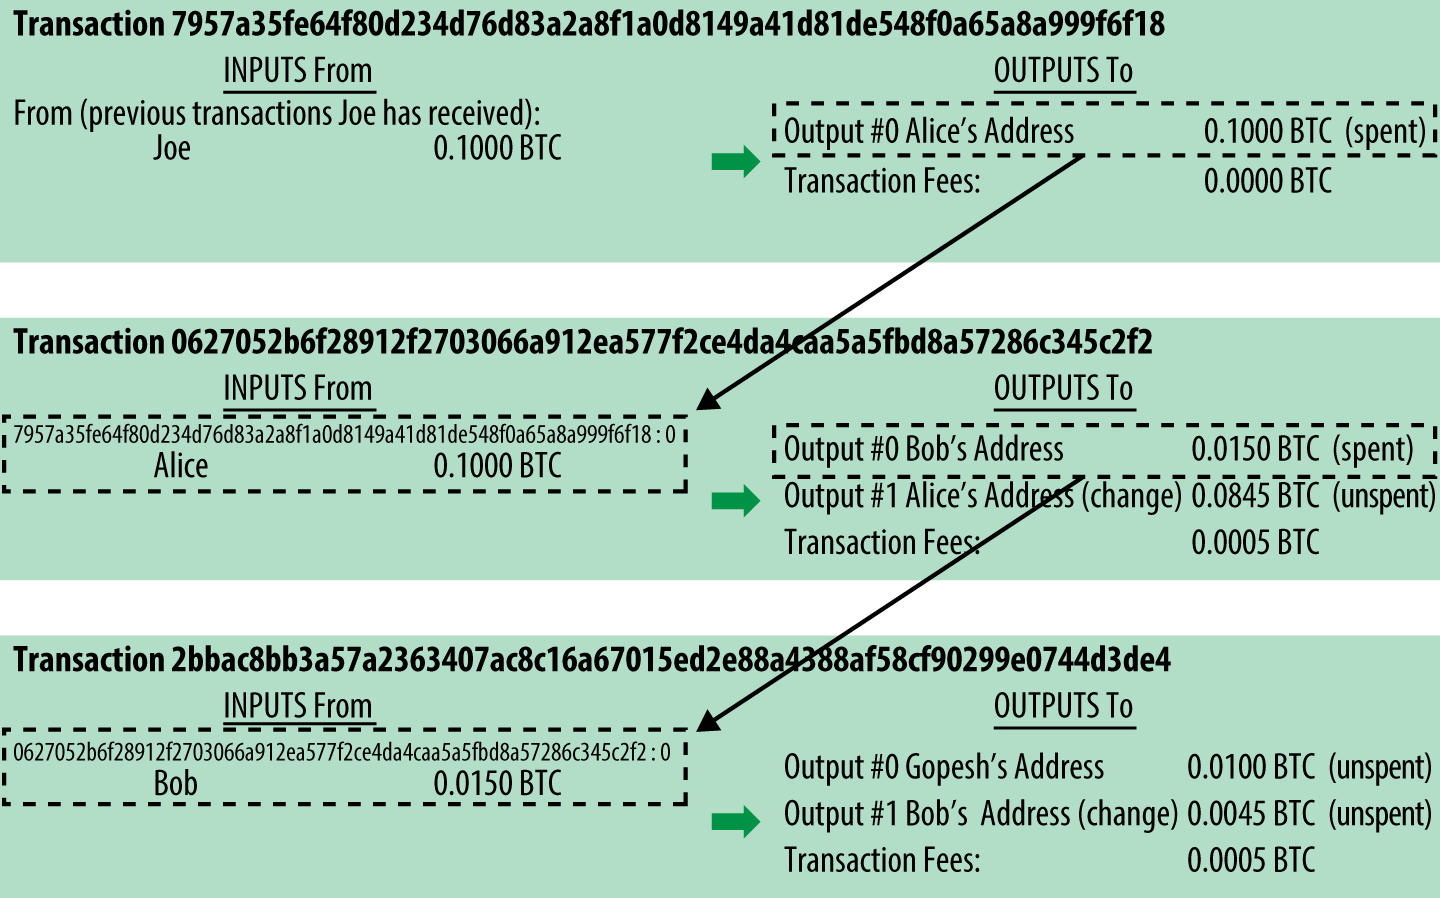
\includegraphics[scale=0.23,clip=false]{pictures/mbc2_0204.png}
  \end{center}

\end{frame}

\begin{frame}\frametitle{Typical transaction: pay somebody and gets the change}

  \begin{center}
    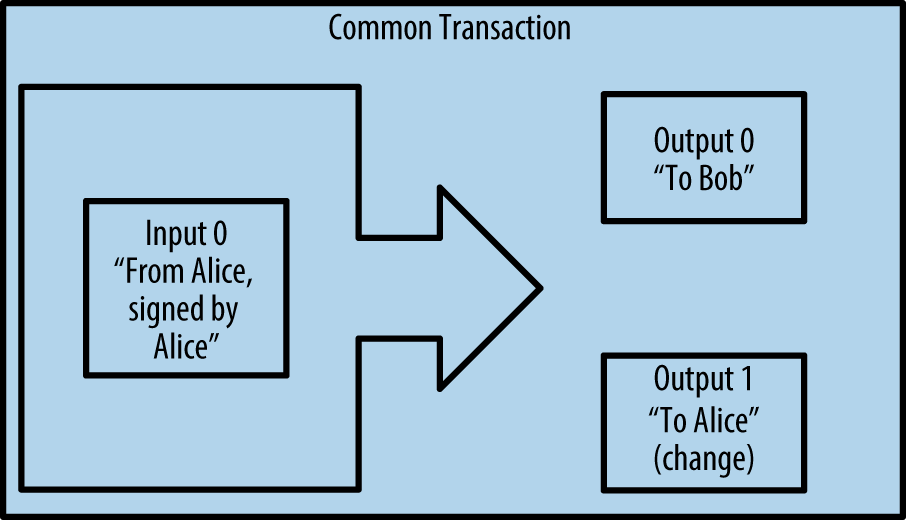
\includegraphics[scale=1.2,clip=false]{pictures/mbc2_0205.png}
  \end{center}

\end{frame}

\begin{frame}\frametitle{Typical transaction: aggregate small notes into a larger one}

  \begin{center}
    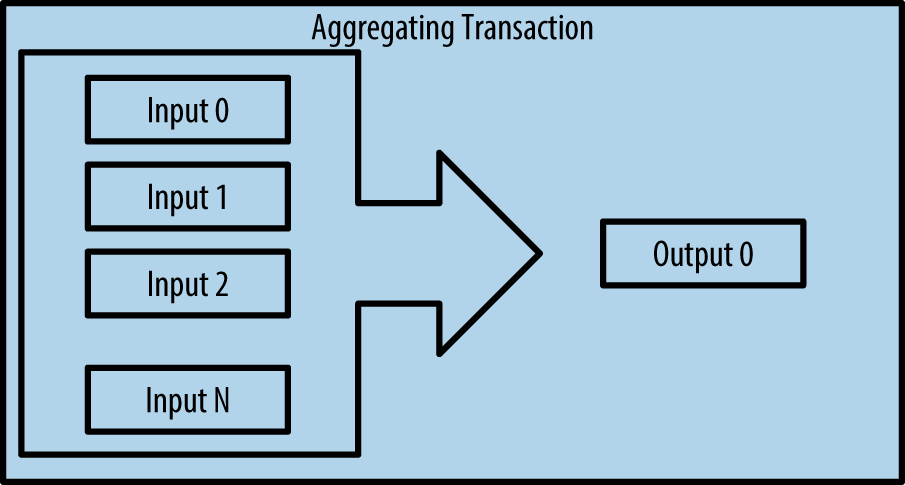
\includegraphics[scale=1.2,clip=false]{pictures/mbc2_0206.png}
  \end{center}

\end{frame}

\begin{frame}\frametitle{Typical transaction: distribution}

  \begin{center}
    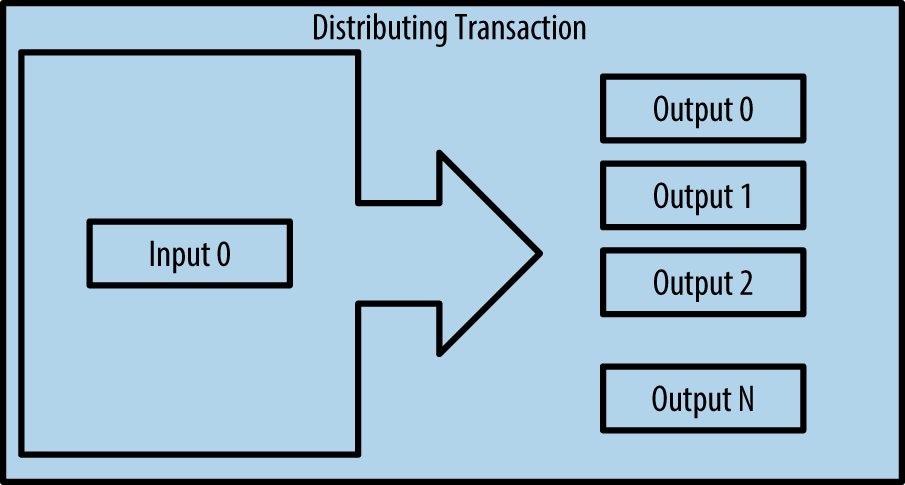
\includegraphics[scale=1.2,clip=false]{pictures/mbc2_0207.png}
  \end{center}

\end{frame}

\begin{frame}\frametitle{A DAG of transactions}

  \begin{center}
    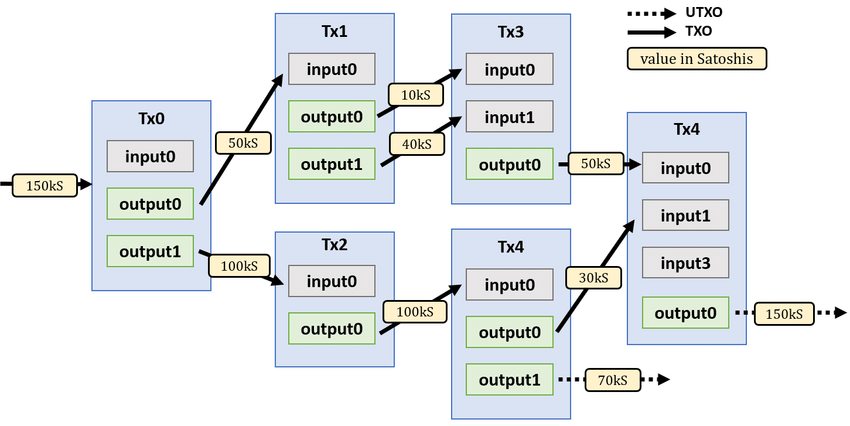
\includegraphics[width=\textwidth,clip=false]{pictures/bitcoin-dag.png}
  \end{center}

\end{frame}

\begin{frame}\frametitle{How Alice's wallet prepares a transaction}

  \begin{enumerate}
  \item Alice's wallet keeps a list of all known unspent outputs for the address
    of Alice
    \begin{itemize}
    \item if it does not know it, it can query the bitcoin network through an API
    \end{itemize}
  \item the wallet selects a subset $\mathit{inputs}$ of the unspent outputs, enough to cover
    the $\mathit{amount}$ of the transaction and signs to prove she's their owner
    \begin{itemize}
    \item any strategy can be applied here
    \end{itemize}
  \item the wallet specifies an output for the destination address of the transaction
    and the $\mathit{amount}\ge 0$ sent to that output
  \item the wallet specifies a second output, normally Alice's address itself, and the
    $\mathit{change}\ge 0$ sent back to Alice
  \item the difference
    \[
    \mathit{fee}=\sum\mathit{inputs}-\mathit{amount}-\mathit{change}\ge 0
    \]
    is the network's reward (and protection) for processing the transaction
  \end{enumerate}

\end{frame}

\begin{frame}\frametitle{How Alice sends the transaction}

  \begin{enumerate}
  \item Alice's wallet sends the bytes of the transaction to a node of the
    bitcoin p2p network
  \item the transaction gets forwarded among all peers (flooding)
  \item the wallet of the destination will very soon see a transaction
    for its address and can assume that it will eventually be processed
    (\alert{unconfirmed transaction})
  \item eventually, around $10$ minutes later,
    the transaction will be processed by the network and
    the wallet of the destination will notice that (\alert{confirmed transaction})
  \item after some time, around one hour, the transaction can be considered
    as definitively processed (\alert{finalized transaction})
  \end{enumerate}

  Merchants can wait for 3, 4 or 5 before handling over the good,
  depending on the relevance of the transaction

\end{frame}

\begin{frame}\frametitle{Miners and Rewards}

  \begin{greenbox}{Miners are (some) nodes of the bitcoin network. They receive, forward
      and aggregate transactions into collectors, called \alert{blocks}}
    When a node creates a new block, it has the right to tag the block
    with a bitcoin address $\mu$, called the \alert{miner}'s address:
    \begin{itemize}
    \item the fees $\phi_1\cdots\phi_n$ of the $n$ transactions in the block go to $\mu$
    \item some amount of money $\iota$ is created out of thin air and goes to $\mu$
    \end{itemize}
  \end{greenbox}

  \bigskip

  \begin{greenbox}{}
    Typically, $\mu$ belongs to the person/organization who owns the machine that runs the node
  \end{greenbox}

  \bigskip

  \begin{greenbox}{}
    $\iota$ is the \alert{inflation}: it is computed through a fixed algorithm that makes it decrease with the time
    and will eventually reach $0$, the day when 21,000,000 total bitcoins will be mined
    \begin{itemize}
    \item[$\Rightarrow$] bitcoin is deflationary
    \end{itemize}
  \end{greenbox}

\end{frame}

\begin{frame}\frametitle{Bitcoin supply over the years}

  \begin{center}
    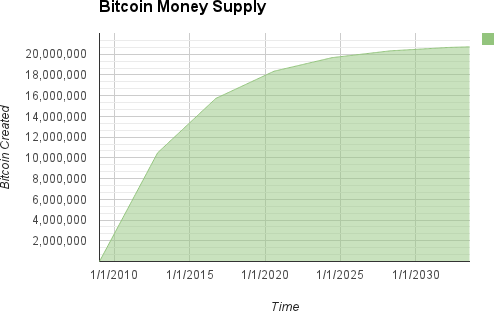
\includegraphics[width=\textwidth,clip=false]{pictures/mbc2_1001.png}
  \end{center}

\end{frame}

\begin{frame}\frametitle{How miners work}

  \begin{enumerate}
    \item Each miner listens the p2p network for new transactions and stores them in a
      temporary area called mempool
    \item when enough new transactions are available in the mempool, it selects some of them
      \begin{itemize}
      \item typically, it selects those with the largest fees, but any other choice is fine: different miners can use different strategies
      \end{itemize}
    \item it builds a new block (\alert{mining}):
      \begin{itemize}
      \item it adds the selected transactions
      \item it adds a special \alert{coinbase transaction} with no inputs, whose only output is $\mu$
        and whose amount is $\iota+\sum_{i=1}^n\phi_i$
      \item it tags the block with a reference to the previous block
      \item it tags the block with its own miner's address $\mu$
      \item it tags the block with a nonce computed by solving an expensive puzzle
      \item if no other miner has been faster, it forwards the new block to all its peers
      \end{itemize}
  \end{enumerate}
\end{frame}

\begin{frame}\frametitle{Block's height, depth and confirmations}

  \begin{center}
    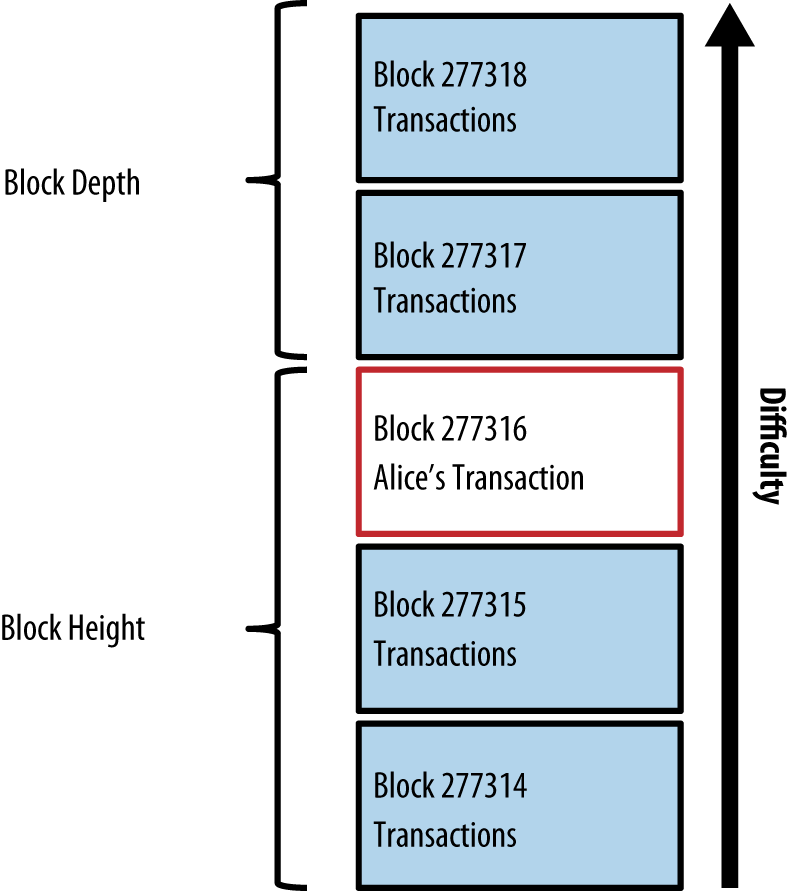
\includegraphics[scale=1,clip=false]{pictures/mbc2_0209.png}
  \end{center}

\end{frame}

\begin{frame}\frametitle{The transaction, again}

  \begin{center}
    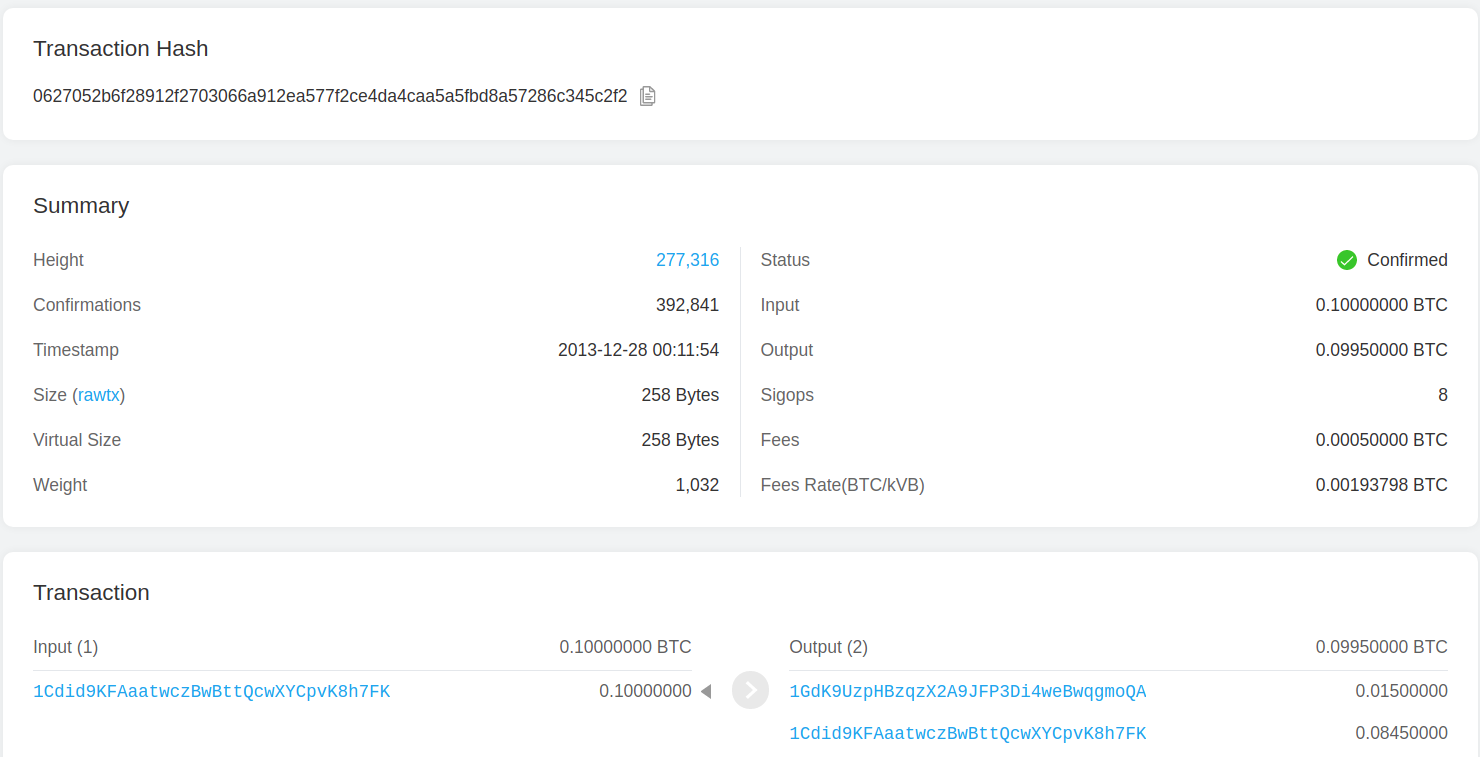
\includegraphics[scale=0.23,clip=false]{pictures/bitcoin-spend.png}
  \end{center}

\end{frame}

\begin{frame}[fragile]\frametitle{The real transaction}

  \begin{center}
    no coins, no senders, no recipients, no balances, no accounts, no addresses
  \end{center}

  {\scriptsize\begin{alltt}
\{
  "vins": [
    \{
      "txid": "7957a35fe64f80d234d76d83a2a8f1a0d8149a41d81de548f0a65a8a999f6f18",
      "vout": 0,
      "unlock": "3045022100884d142d86652a3f47... 0484ecc0d46f..."
    \}
  ],
  "vouts": [
    \{
      "value": 0.01500000,
      "lock": "DUP HASH160 ab68025513c3dbd2f7b92a94e0581f5d50f654e7 
               EQUALVERIFY CHECKSIG"
    \},
    \{
      "value": 0.08450000,
      "lock": "DUP HASH160 7f9b1a7fb68d60c536c2fd8aeaa53a8f3cc025a8
               EQUALVERIFY CHECKSIG"
    \}
  ]
\}
\end{alltt}}

\end{frame}

\begin{frame}[fragile]\frametitle{The real transaction}

  \begin{center}
    two new UTXOs (unspent transaction outputs)
  \end{center}

  {\scriptsize\begin{alltt}
\{
  "vins": [
    \{
      "txid": "7957a35fe64f80d234d76d83a2a8f1a0d8149a41d81de548f0a65a8a999f6f18",
      "vout": 0,
      "unlock": "3045022100884d142d86652a3f47... 0484ecc0d46f..."
    \}
  ],
  \color{red}{"vouts": [
    \{
      "value": 0.01500000,
      "lock": "DUP HASH160 ab68025513c3dbd2f7b92a94e0581f5d50f654e7
               EQUALVERIFY CHECKSIG"
    \},
    \{
      "value": 0.08450000,
      "lock": "DUP HASH160 7f9b1a7fb68d60c536c2fd8aeaa53a8f3cc025a8
               EQUALVERIFY CHECKSIG",
    \}
  ]}
\}
\end{alltt}}

\end{frame}

\begin{frame}[fragile]\frametitle{The real transaction}

  \begin{center}
    reference to an old UTXO (soon to be TXO)
  \end{center}

  {\scriptsize\begin{alltt}
\{
  \alert{"vins": [
    \{
      "txid": "7957a35fe64f80d234d76d83a2a8f1a0d8149a41d81de548f0a65a8a999f6f18",
      "vout": 0,
      "unlock": "3045022100884d142d86652a3f47... 0484ecc0d46f..."
    \}
  ]},
  "vouts": [
    \{
      "value": 0.01500000,
      "lock": "DUP HASH160 ab68025513c3dbd2f7b92a94e0581f5d50f654e7
               EQUALVERIFY CHECKSIG"
    \},
    \{
      "value": 0.08450000,
      "lock": "DUP HASH160 7f9b1a7fb68d60c536c2fd8aeaa53a8f3cc025a8
               EQUALVERIFY CHECKSIG"
    \}
  ]
\}
\end{alltt}}

\end{frame}

\begin{frame}[fragile]\frametitle{The real transaction}

  \begin{center}
    the amount of the first new UTXO (in satoshis)
  \end{center}

  {\scriptsize\begin{alltt}
\{
  "vins": [
    \{
      "txid": "7957a35fe64f80d234d76d83a2a8f1a0d8149a41d81de548f0a65a8a999f6f18",
      "vout": 0,
      "unlock": "3045022100884d142d86652a3f47... 0484ecc0d46f..."
    \}
  ],
  "vouts": [
    \{
      \alert{"value": 0.01500000},
      "lock": "DUP HASH160 ab68025513c3dbd2f7b92a94e0581f5d50f654e7
               EQUALVERIFY CHECKSIG"
    \},
    \{
      "value": 0.08450000,
      "lock": "DUP HASH160 7f9b1a7fb68d60c536c2fd8aeaa53a8f3cc025a8
               EQUALVERIFY CHECKSIG"
    \}
  ]
\}
\end{alltt}}

\end{frame}

\begin{frame}[fragile]\frametitle{The real transaction}

  \begin{center}
    the unlocking or witness script of the first new UTXO (crypto-puzzle)
  \end{center}

  {\scriptsize\begin{alltt}
\{
  "vins": [
    \{
      "txid": "7957a35fe64f80d234d76d83a2a8f1a0d8149a41d81de548f0a65a8a999f6f18",
      "vout": 0,
      "unlock": "3045022100884d142d86652a3f47... 0484ecc0d46f..."
    \}
  ],
  "vouts": [
    \{
      "value": 0.01500000,
      \alert{"lock": "DUP HASH160 ab68025513c3dbd2f7b92a94e0581f5d50f654e7
               EQUALVERIFY CHECKSIG"}
    \},
    \{
      "value": 0.08450000,
      "lock": "DUP HASH160 7f9b1a7fb68d60c536c2fd8aeaa53a8f3cc025a8
               EQUALVERIFY CHECKSIG"
    \}
  ]
\}
\end{alltt}}

\end{frame}

\begin{frame}[fragile]\frametitle{The real transaction}

  \begin{center}
    the hash of the transaction whose $\mathtt{vout}^{\mathit{th}}$ UTXO is being spent
  \end{center}

  {\scriptsize\begin{alltt}
\{
  "vins": [
    \{
      \alert{"txid": "7957a35fe64f80d234d76d83a2a8f1a0d8149a41d81de548f0a65a8a999f6f18",
      "vout": 0},
      "unlock": "3045022100884d142d86652a3f47... 0484ecc0d46f..."
    \}
  ],
  "vouts": [
    \{
      "value": 0.01500000,
      "lock": "DUP HASH160 ab68025513c3dbd2f7b92a94e0581f5d50f654e7
               EQUALVERIFY CHECKSIG"
    \},
    \{
      "value": 0.08450000,
      "lock": "DUP HASH160 7f9b1a7fb68d60c536c2fd8aeaa53a8f3cc025a8
               EQUALVERIFY CHECKSIG"
    \}
  ]
\}
\end{alltt}}

\end{frame}

\begin{frame}[fragile]\frametitle{The real transaction}

  \begin{center}
    the unlocking script (usually digital signature + public key)
  \end{center}

  {\scriptsize\begin{alltt}
\{
  "vins": [
    \{
      "txid": "7957a35fe64f80d234d76d83a2a8f1a0d8149a41d81de548f0a65a8a999f6f18",
      "vout": 0,
      \alert{"unlock": "3045022100884d142d86652a3f47... 0484ecc0d46f..."}
    \}
  ],
  "vouts": [
    \{
      "value": 0.01500000,
      "lock": "DUP HASH160 ab68025513c3dbd2f7b92a94e0581f5d50f654e7
               EQUALVERIFY CHECKSIG"
    \},
    \{
      "value": 0.08450000,
      "lock": "DUP HASH160 7f9b1a7fb68d60c536c2fd8aeaa53a8f3cc025a8
               EQUALVERIFY CHECKSIG",
    \}
  ]
\}
\end{alltt}}

\end{frame}

\begin{frame}[fragile]\frametitle{The real transaction}

  \begin{center}
    scripts are written in the Script programming language
  \end{center}

  {\scriptsize\begin{alltt}
\{
  "vins": [
    \{
      "txid": "7957a35fe64f80d234d76d83a2a8f1a0d8149a41d81de548f0a65a8a999f6f18",
      "vout": 0,
      "unlock": \alert{"3045022100884d142d86652a3f47... 0484ecc0d46f..."}
    \}
  ],
  "vouts": [
    \{
      "value": 0.01500000,
      "lock": \alert{"DUP HASH160 ab68025513c3dbd2f7b92a94e0581f5d50f654e7
               EQUALVERIFY CHECKSIG"}
    \},
    \{
      "value": 0.08450000,
      "lock": \alert{"DUP HASH160 7f9b1a7fb68d60c536c2fd8aeaa53a8f3cc025a8
               EQUALVERIFY CHECKSIG"}
    \}
  ]
\}
\end{alltt}}

\end{frame}

\begin{frame}\frametitle{The Script programming language}

  \begin{greenbox}{Reverse-polish stack-based stateless language}
    \begin{itemize}
    \item[{
\includegraphics[scale=0.03]{pictures/check.png}}] sequence
    \item[{
\includegraphics[scale=0.03]{pictures/check.png}}] conditional
    \item[{
\includegraphics[scale=0.0135]{pictures/uncheck.png}}] repetition
    \end{itemize}

    \begin{center}
      \alert{$\Rightarrow$ Turing incomplete}
    \end{center}

  \end{greenbox}

  \bigskip

  \begin{greenbox}{Why Turing incomplete?}
    \begin{enumerate}
    \item predictable execution time
    \item guaranteed termination
    \end{enumerate}

    \begin{center}
      denial-of-service attacks are impossible \emph{at language level}
    \end{center}

  \end{greenbox}

\end{frame}

\begin{frame}\frametitle{Script validity}

  \begin{greenbox}{}
    A program in the Script language is \alert{valid} if its execution
    does not stop with failure and terminates with a stack whose topmost element is \texttt{TRUE}
  \end{greenbox}

  \bigskip

  \begin{greenbox}{Execution proceeds left-to-right}
    Let us execute \texttt{2 3 ADD 5 EQUAL} to see if it's valid
  \end{greenbox}

\end{frame}

\begin{frame}\frametitle{\texttt{2 3 ADD 5 EQUAL}}

  \begin{center}
    \only<1>{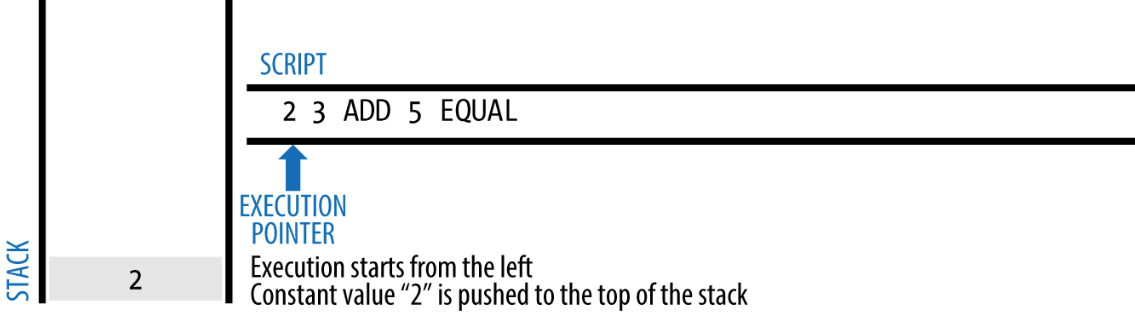
\includegraphics[width=\textwidth,clip=false]{pictures/stack1.png}}
    \only<2>{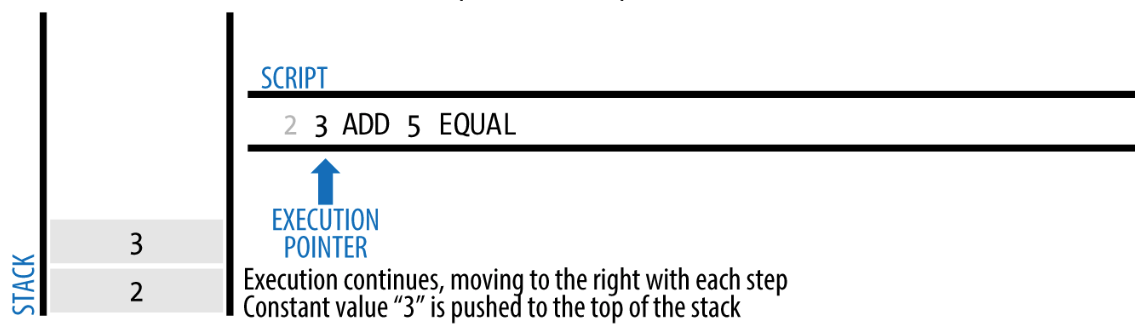
\includegraphics[width=\textwidth,clip=false]{pictures/stack2.png}}
    \only<3>{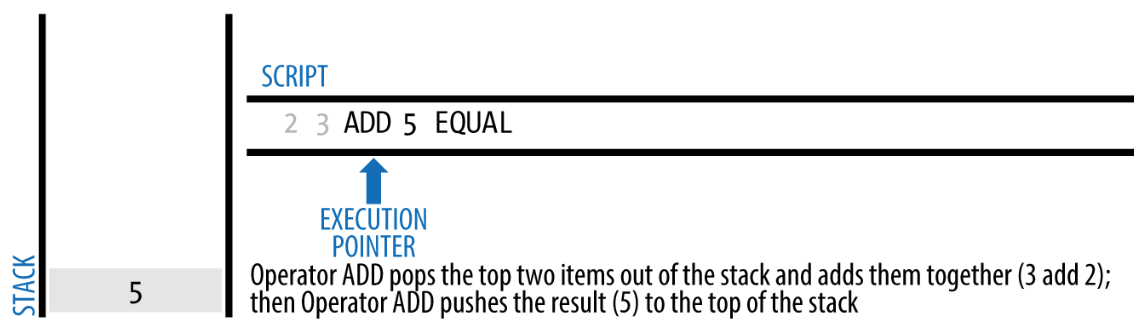
\includegraphics[width=\textwidth,clip=false]{pictures/stack3.png}}
    \only<4>{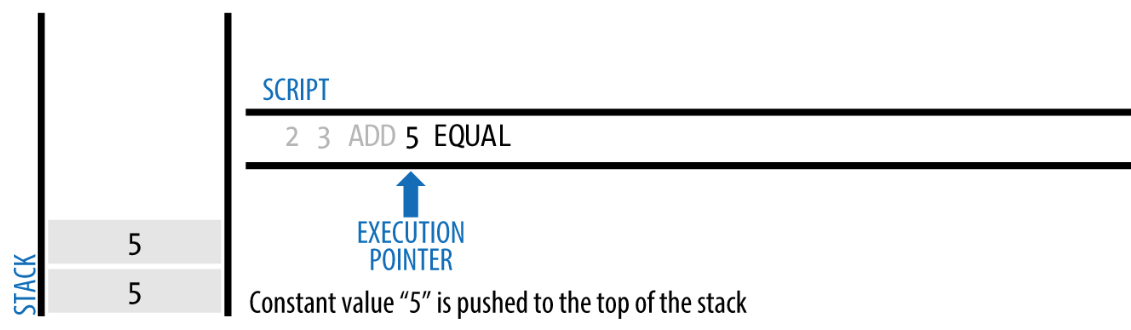
\includegraphics[width=\textwidth,clip=false]{pictures/stack4.png}}
    \only<5>{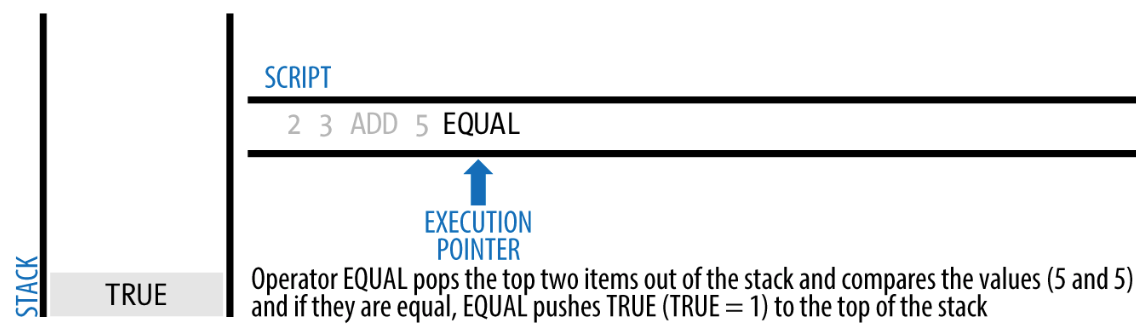
\includegraphics[width=\textwidth,clip=false]{pictures/stack5.png}}
  \end{center}

  \begin{center}
    \only<5>{The program is valid!}
  \end{center}

\end{frame}

\begin{frame}\frametitle{Other examples of (in-)valid scripts}

  \begin{greenbox}{These are all valid}
    \begin{itemize}
    \item \texttt{TRUE}
    \item \texttt{FALSE TRUE}
    \item \texttt{2 7 ADD 3 SUB 1 ADD 7 EQUAL}
    \item \texttt{2 7 EQUAL IF FALSE ELSE TRUE ENDIF}
    \end{itemize}
  \end{greenbox}

  \bigskip

  \begin{greenbox}{These are all invalid}
    \begin{itemize}
    \item \texttt{FALSE}
    \item \texttt{2 7 EQUAL}
    \item \texttt{2 7 EQUAL IF TRUE ELSE FALSE ENDIF}
    \item \texttt{2 7 EQUAL TRUE ENDIF}
    \end{itemize}
  \end{greenbox}

\end{frame}

\begin{frame}[fragile]\frametitle{The validation algorithm for bitcoin transactions}

{\scriptsize\begin{alltt}
previous_tx = \{ // this transaction has hash H
  "vins": .....
  "vouts": [ \{ "value": .....,     "lock": "....." \}, ..... ]
\}

tx = \{
  "vins": [ \{ "txid": H,     "vout": .....,     "unlock": "....." \}, ..... ],
  "vouts": .....
\}
\end{alltt}}

    {\small\begin{alltt}
    boolean is_valid(Transaction tx) \{
      for each (txid, vout, unlock) in tx.vins
        previous_tx = \alert{get_transaction}(txid)
        lock = previous_tx.vouts[vout].lock
        if ({\color{blue}{unlock lock}} is invalid)
          return false

      return true
    \}
    \end{alltt}}

\end{frame}

\begin{frame}[fragile]\frametitle{The typical P2PKH script (\emph{pay to publickey hash})}

\begin{greenbox}{``I want to send some value to \<address>''}
{\scriptsize\begin{alltt}
previous_tx = \{ // this transaction has hash H
  "vins": .....
  "vouts": [\{ "value": ..., "lock": {\color{blue}{DUP HASH160 <address> EQUALVERIFY CHECKSIG}} \},
            .....]
\}
\end{alltt}}
\end{greenbox}

\bigskip

\begin{greenbox}{``I'm \<address>, here is my signature, use that value''}
{\scriptsize\begin{alltt}
tx = \{
  "vins": [ \{ "txid": H,   "vout": .....,   "unlock": {\color{blue}{<sig> <PubK>}}\}, ..... ],
  "vouts": .....
\}
\end{alltt}}
\end{greenbox}

\bigskip

\begin{greenbox}{\<unlock lock>}
  \begin{center}
    \texttt{<sig> <PubK> DUP HASH160 <address> EQUALVERIFY CHECKSIG}
  \end{center}
\end{greenbox}

The bitcoin \<address> is often referred to as \<PublicKHash>

\end{frame}

\begin{frame}\frametitle{\texttt{<sig> <PubK> DUP HASH160 <address> EQUALVERIFY CHECKSIG}}

  \begin{center}
    \only<1>{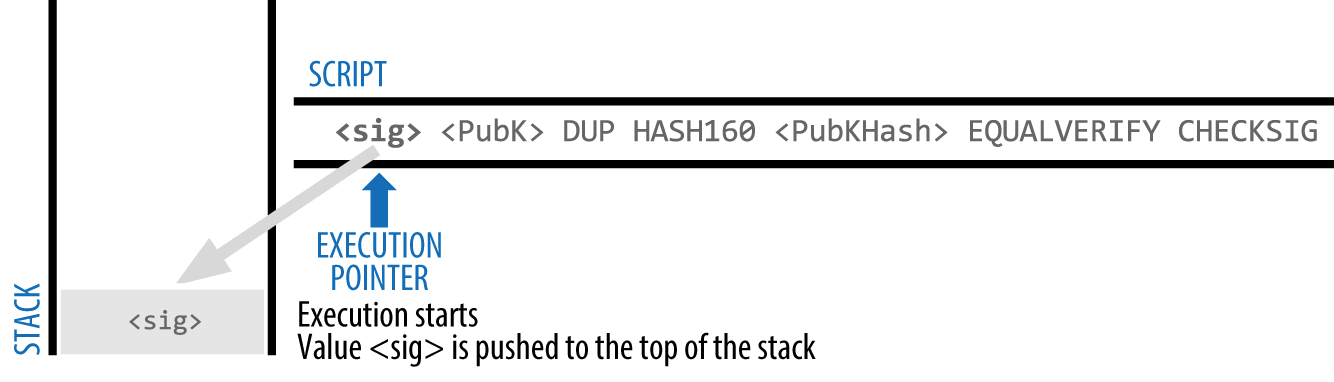
\includegraphics[width=\textwidth,clip=false]{pictures/p2pkh1.png}}
    \only<2>{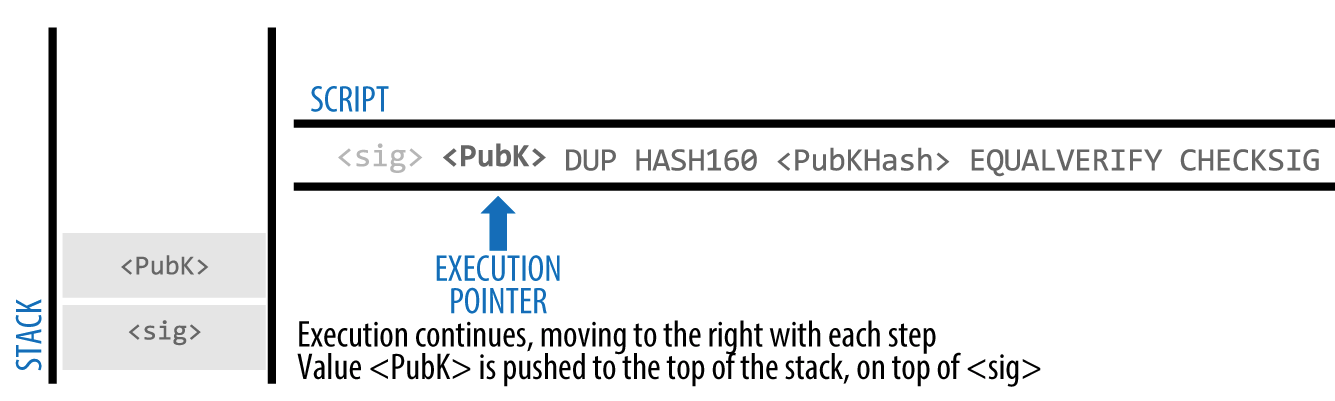
\includegraphics[width=\textwidth,clip=false]{pictures/p2pkh2.png}}
    \only<3>{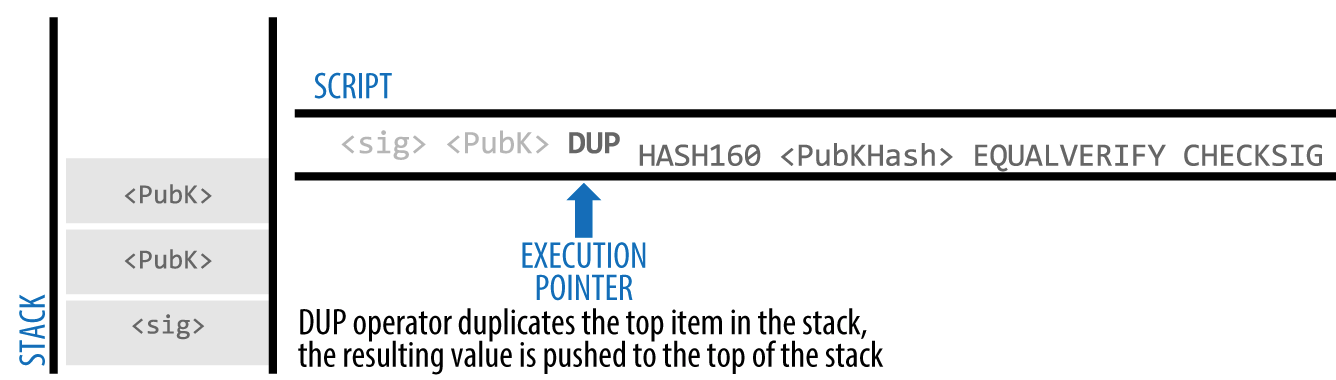
\includegraphics[width=\textwidth,clip=false]{pictures/p2pkh3.png}}
    \only<4>{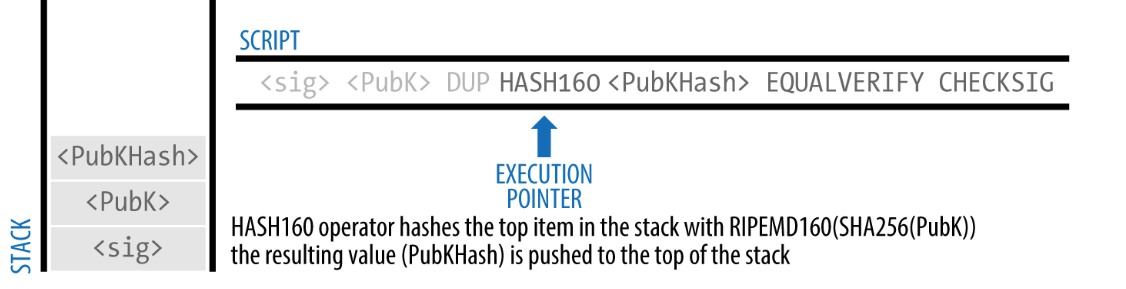
\includegraphics[width=\textwidth,clip=false]{pictures/p2pkh4.png}}
    \only<5>{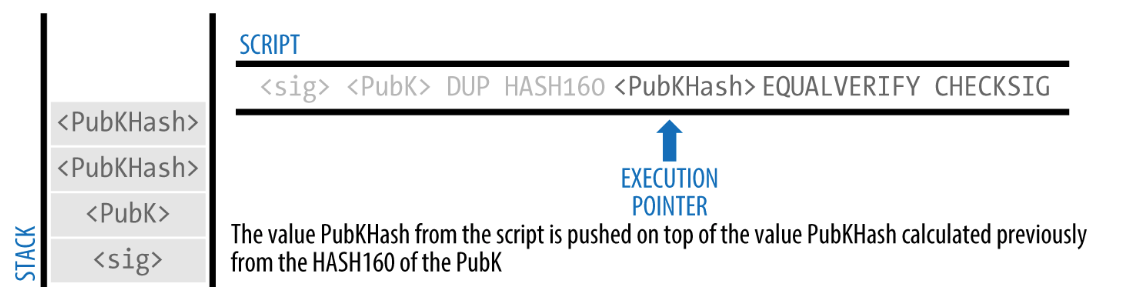
\includegraphics[width=\textwidth,clip=false]{pictures/p2pkh5.png}}
    \only<6-7>{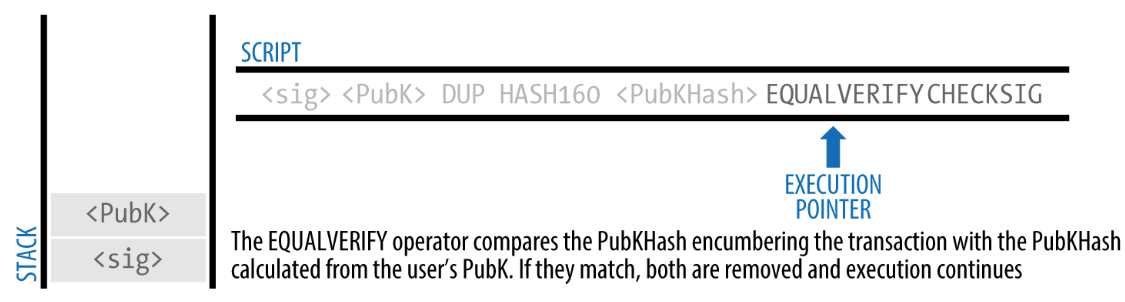
\includegraphics[width=\textwidth,clip=false]{pictures/p2pkh6.png}}+
    \only<8>{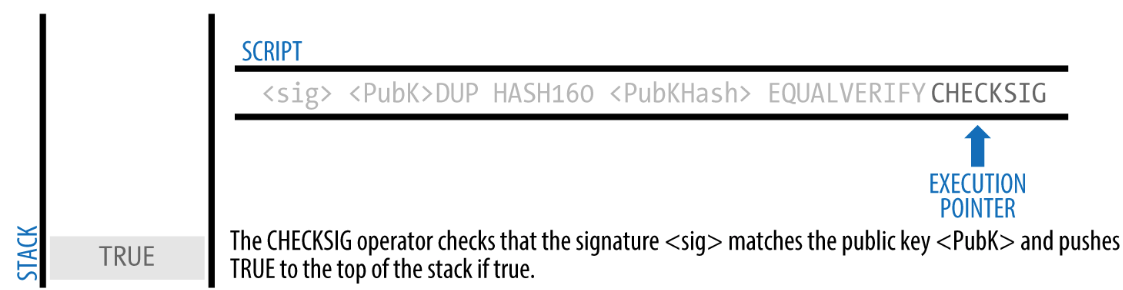
\includegraphics[width=\textwidth,clip=false]{pictures/p2pkh7.png}}
  \end{center}

  \uncover<7>{
    \begin{greenbox}{}
      \<CHECKSIG> verifies that \<sig> is a signature of the transaction
      generated by using the private key corresponsing to \<pubK>
    \end{greenbox}
  }

  \uncover<8>{
    \begin{center}
      This script gives proof of ownership!
    \end{center}
  }

\end{frame}

\begin{frame}\frametitle{Headers, blocks and blockchain, genesis block}

  \begin{center}
    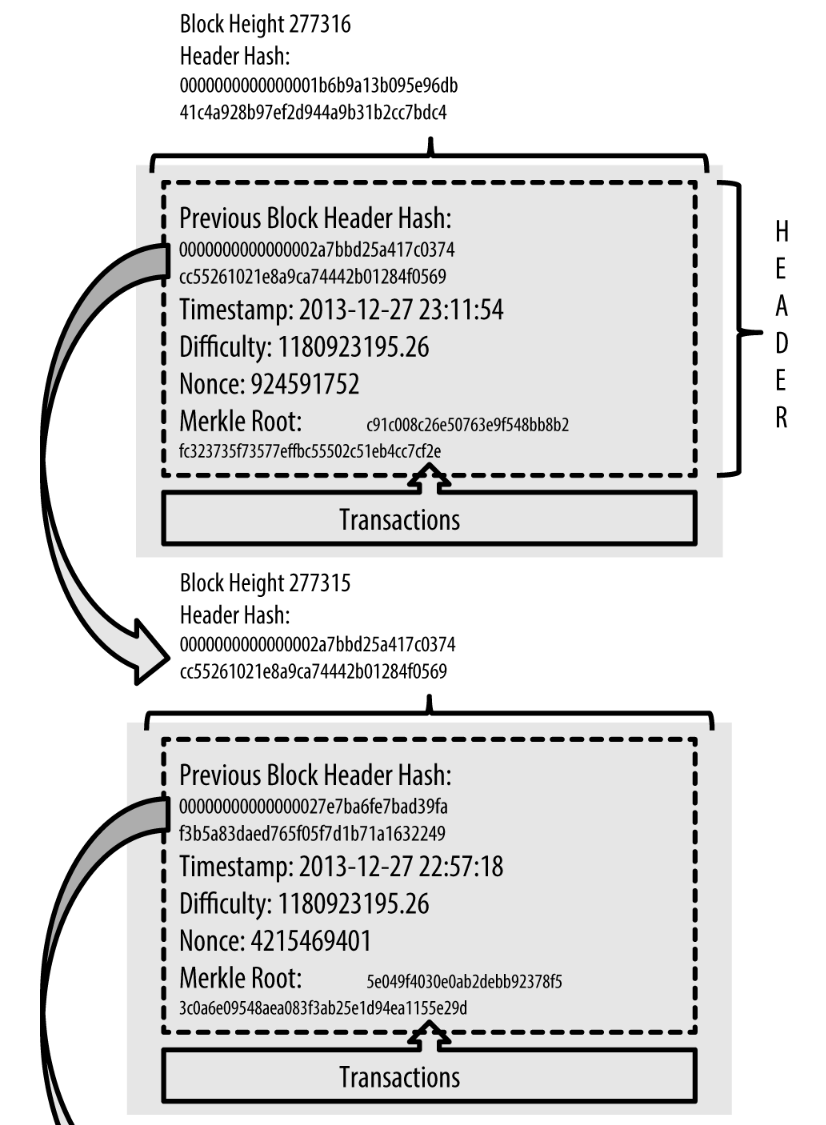
\includegraphics[scale=0.2,clip=false]{pictures/bitcoin-blocks.png}
  \end{center}

\end{frame}

\begin{frame}\frametitle{The header contains the hash of all transactions in the block (Merkle root)}

  \begin{center}
    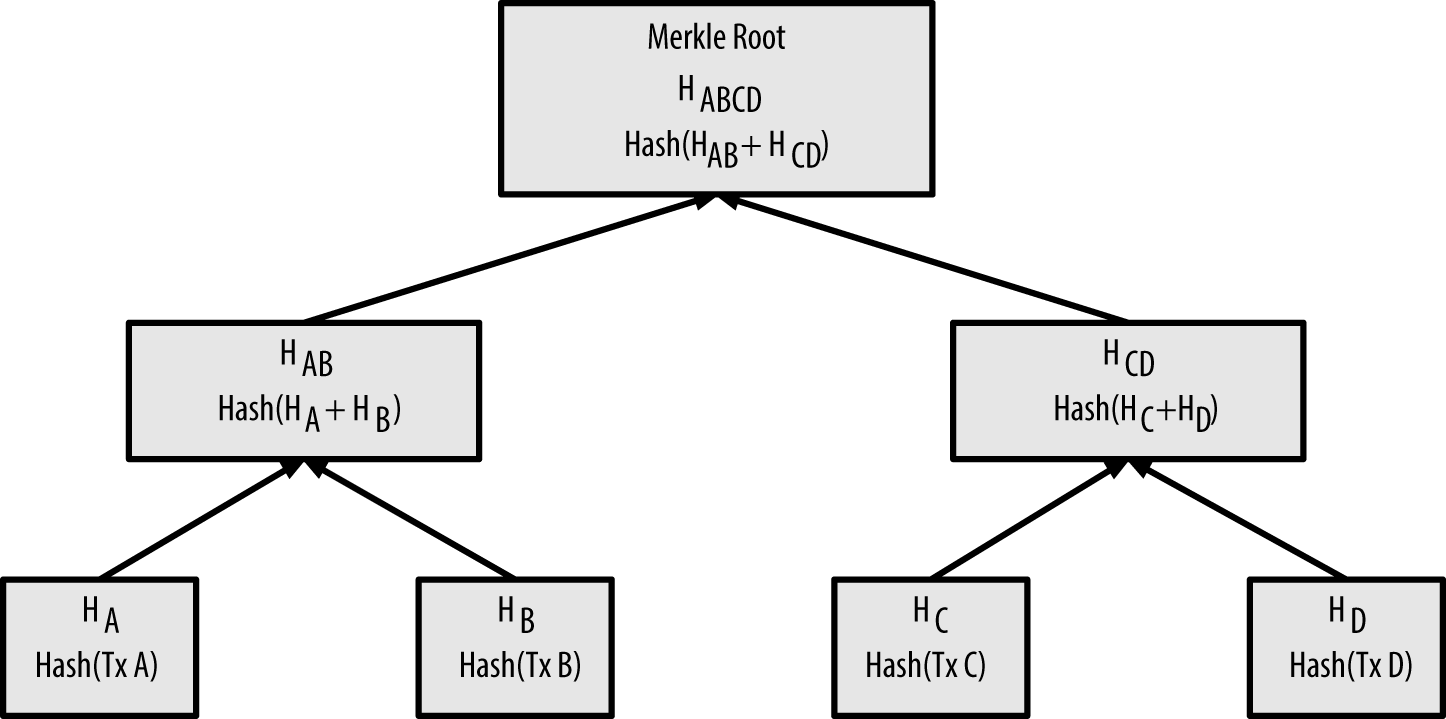
\includegraphics[width=\textwidth,clip=false]{pictures/mbc2_0902.png}
  \end{center}

\end{frame}

\begin{frame}\frametitle{Merkle trees provide an efficient inclusion test}

  \begin{center}
    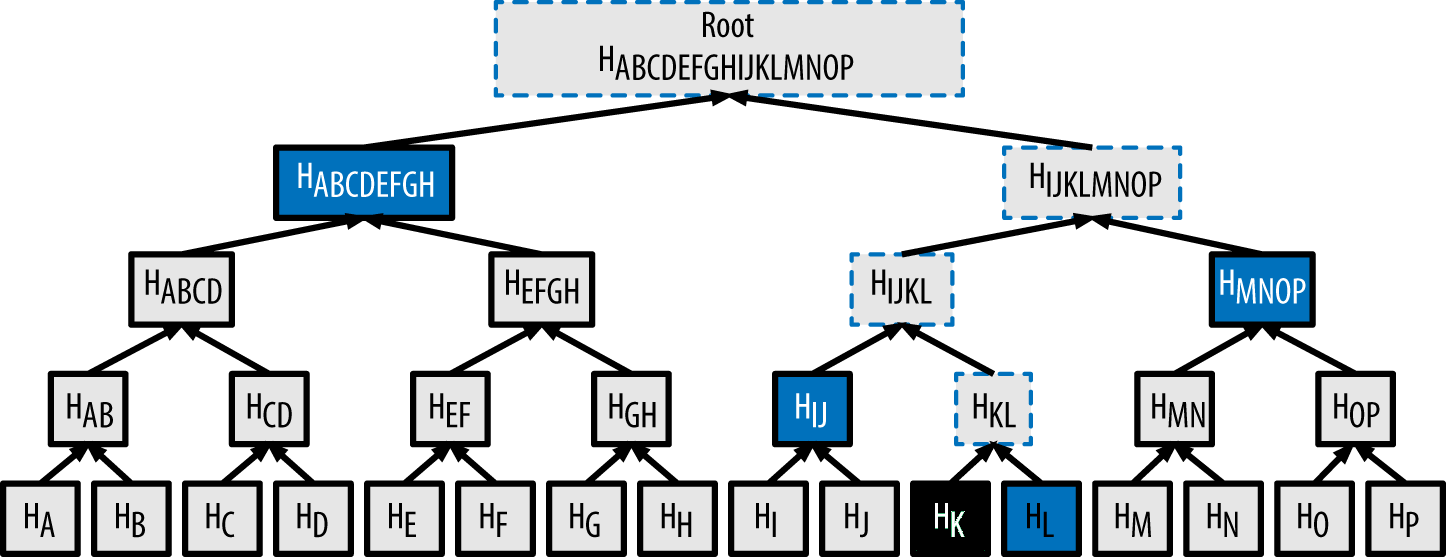
\includegraphics[width=\textwidth,clip=false]{pictures/mbc2_0905.png}
  \end{center}

  \begin{greenbox}{I know the root hash and want to know if the {\color{black}black $H_K$} is included}
    The {\color{blue}four blue hashes} can be given to me as that proof of inclusion
    (\emph{authentication path})
  \end{greenbox}

\end{frame}

\begin{frame}\frametitle{Mining}

  \begin{center}
    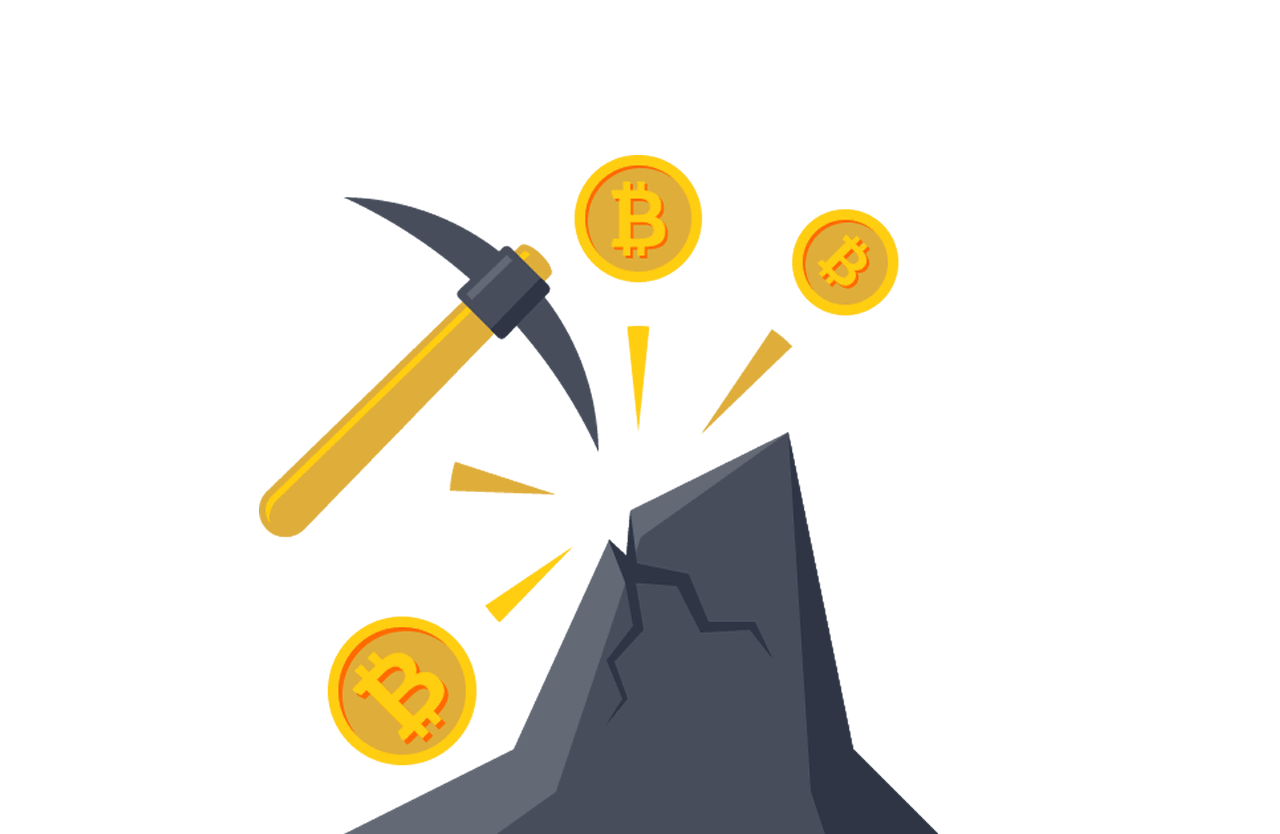
\includegraphics[scale=0.1,clip=false]{pictures/mining.png}
  \end{center}

  \bigskip

  \begin{greenbox}{The vision of the miner}
    The goal of mining is to mint new coins and earn money
  \end{greenbox}

  \bigskip

  \begin{greenbox}{The vision of Nakamoto}
    The goal of mining is to secure the bitcoin network
  \end{greenbox}

\end{frame}

\begin{frame}\frametitle{Miners can only mine correct blocks}

  \begin{greenbox}{New valid block = it respects the {\color{pink}{consensus rules}}}
    \begin{itemize}
    \item the structure of data in the header and transactions must be correct
    \item transactions have at least one input (but for coinbase transactions)
    \item transactions have at least one output
    \item transactions do not create money (but for coinbase transactions)
    \item coinbase transactions have a correct reward
    \item transactions are all valid (their unlocking scripts match the corresponsing locking scripts)
    \item transaction inputs refer to unspent UTXO only
      (\alert{no double-spending inside the same history})
    \item \ldots
    \end{itemize}
  \end{greenbox}

  \medskip

  \begin{redbox}{}
    \begin{center}
      But what about fairness?
    \end{center}
  \end{redbox}

\end{frame}

\begin{frame}\frametitle{How to kill a dictator}

  \begin{greenbox}{Without proof of work}
    A single node dictates the history of the blockchain
    if it is faster than \emph{each} other node
  \end{greenbox}

  \pause
  \bigskip
  \bigskip

  \begin{greenbox}{With proof of work}
    A single node dictates the history of the blockchain
    if it is faster than \emph{the sum of all} other nodes
  \end{greenbox}

\end{frame}

\begin{frame}\frametitle{Proof-of-work (PoW)}

  \begin{greenbox}{Add the following consensus rule}
    The hash of valid blocks is smaller than
    a given constant $\mathit{difficulty}$
  \end{greenbox}

  \bigskip

  \begin{greenbox}{Miners must work hard now}
    \begin{enumerate}
    \item build a new block
    \item set the nonce field of its header to a random value
    \item compute the hash $h$ of the header
    \item if $h < \mathit{difficulty}$ stop
    \item otherwise, go back to step 2 and try again
    \end{enumerate}
  \end{greenbox}

  \bigskip

  \begin{itemize}
  \item the header of the resulting block is the PoW
  \item the time to solve this puzzle is inversely proportional to $\mathit{difficulty}$
  \item the algorithm can be easily run in parallel
  \end{itemize}

\end{frame}

\begin{frame}\frametitle{The blockchain grows}

  \begin{itemize}
  \item the miner creates a new block on top of the main history
  \item the miner receives a valid new block from a peer
    \begin{itemize}
    \item whose parent is the top of the main history, or
    \item whose parent is another block of the blockchain (fork), or
    \item whose parent is unknown to the miner (orphan block)
    \end{itemize}
  \item in case of fork, the main history is the longest one, but the miner keeps all histories,
    in case they might become the new main history in the future
  \end{itemize}
  
\end{frame}

\begin{frame}\frametitle{Fork: all nodes start with the same vision}

  \begin{center}
    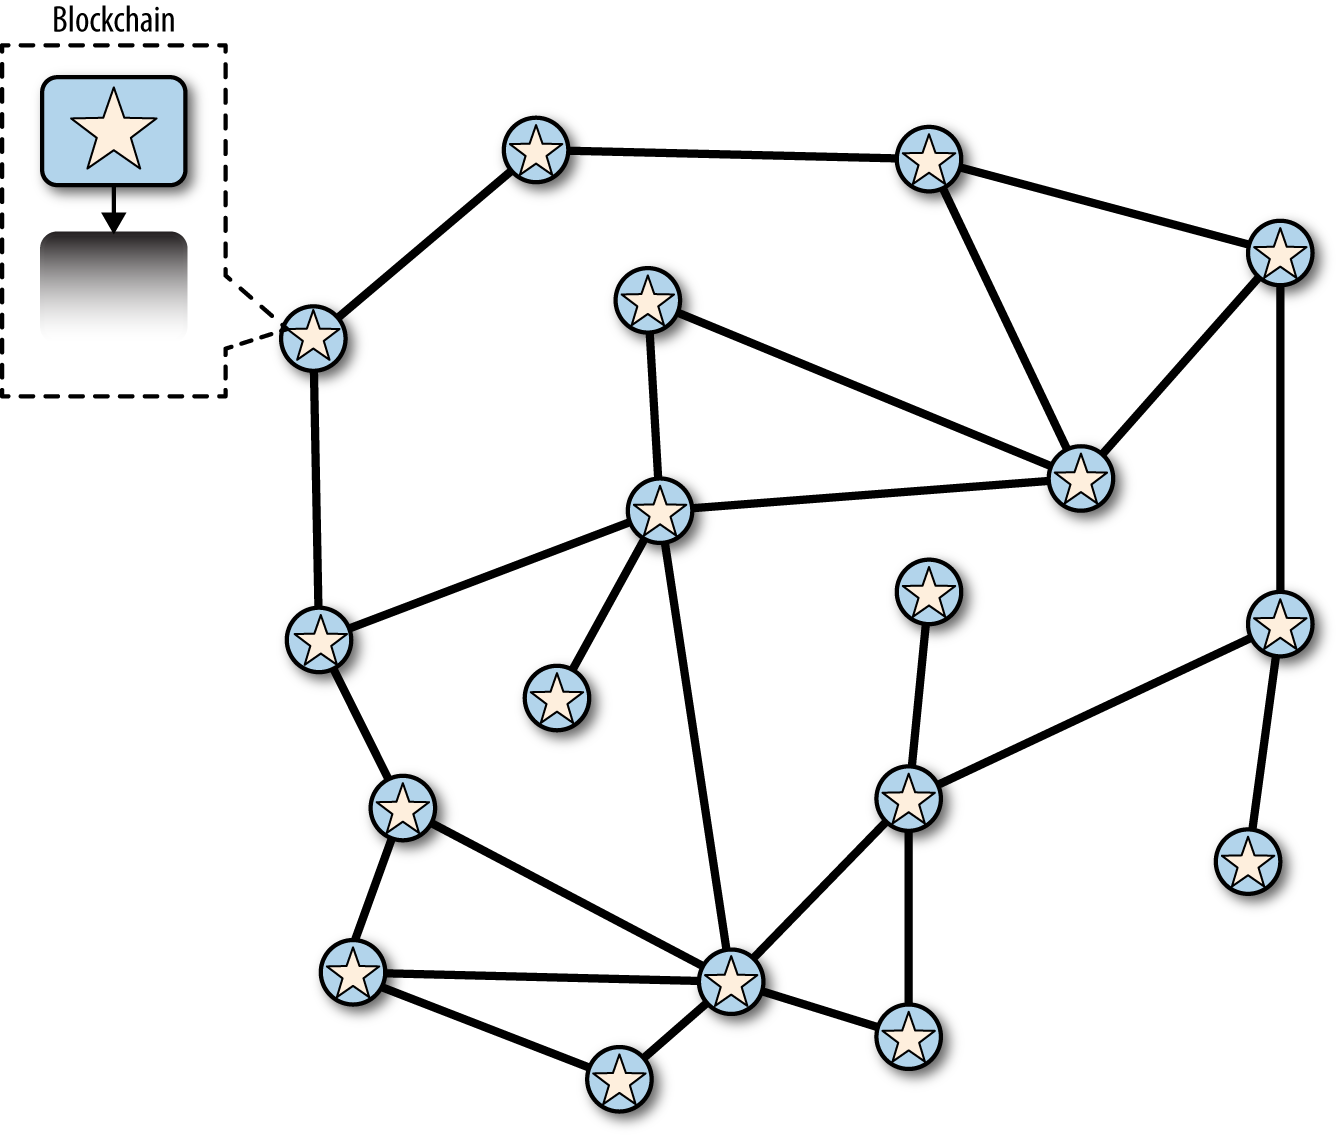
\includegraphics[scale=0.8,clip=false]{pictures/mbc2_1002.png}
  \end{center}

\end{frame}

\begin{frame}\frametitle{Fork: two nodes expand the blockchain simultaneously}

  \begin{center}
    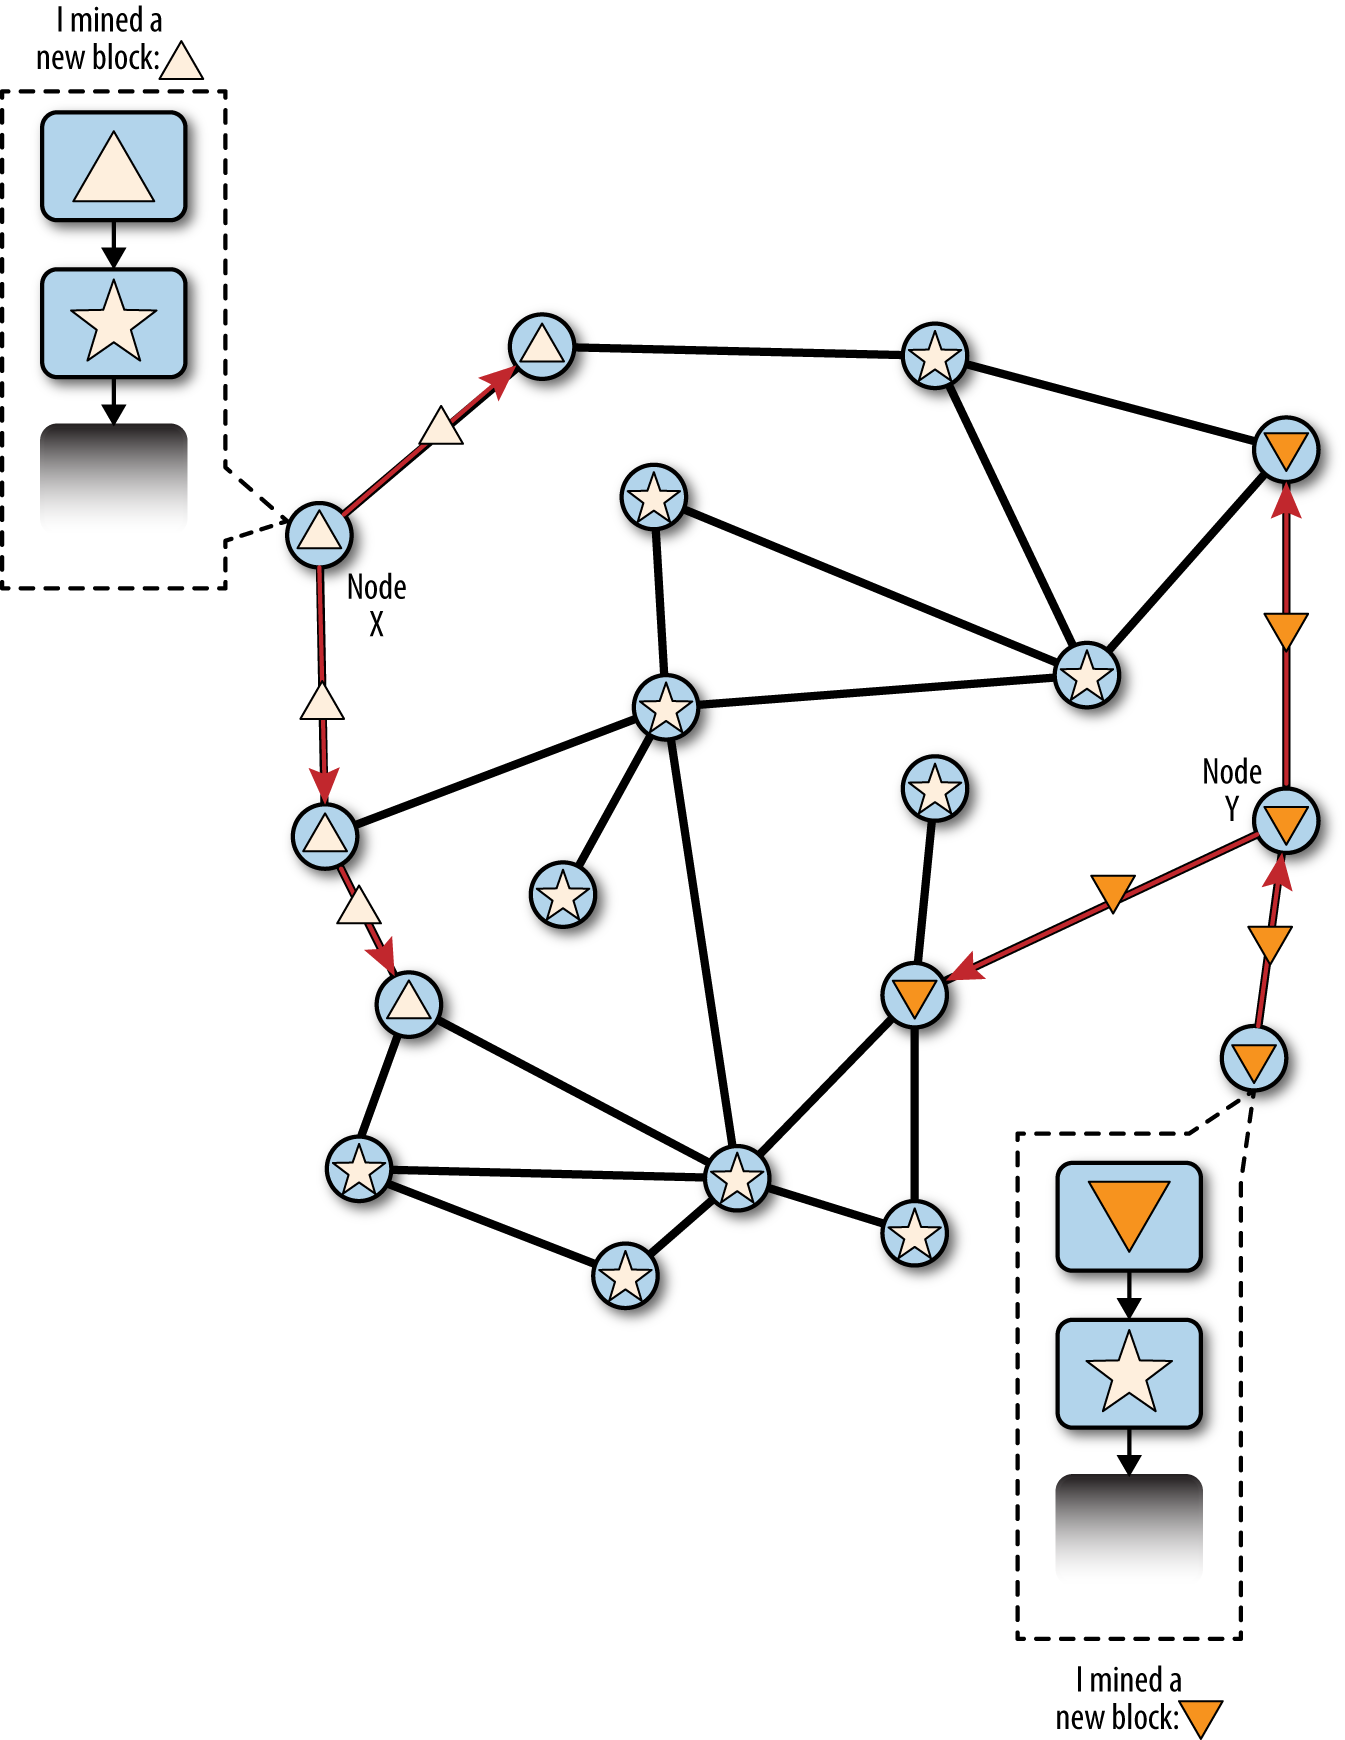
\includegraphics[scale=0.53,clip=false]{pictures/mbc2_1003.png}
  \end{center}

\end{frame}

\begin{frame}\frametitle{Fork: the network is split}

  \begin{center}
    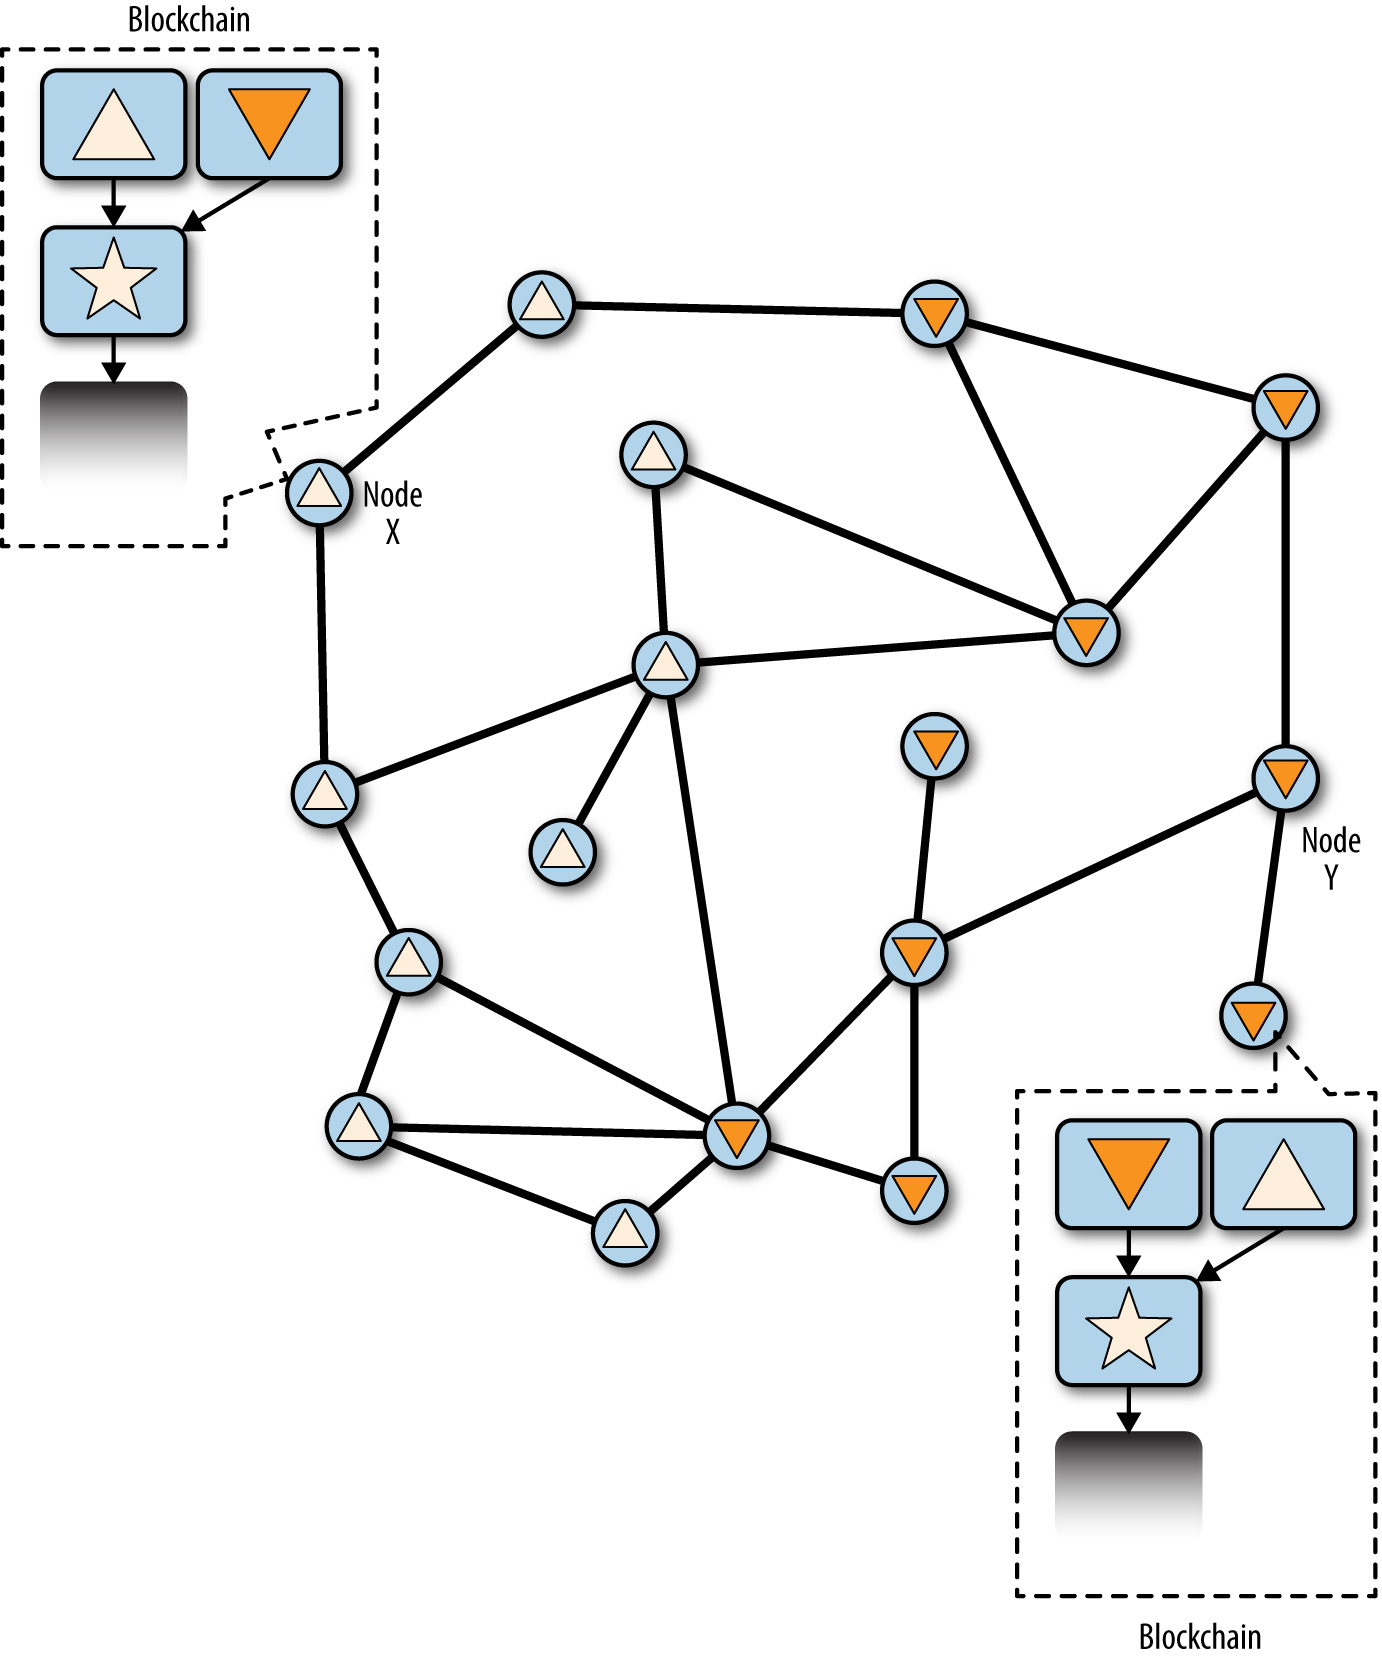
\includegraphics[scale=0.56,clip=false]{pictures/mbc2_1004.png}
  \end{center}

\end{frame}

\begin{frame}\frametitle{Fork: either chain is expanded further}

  \begin{center}
    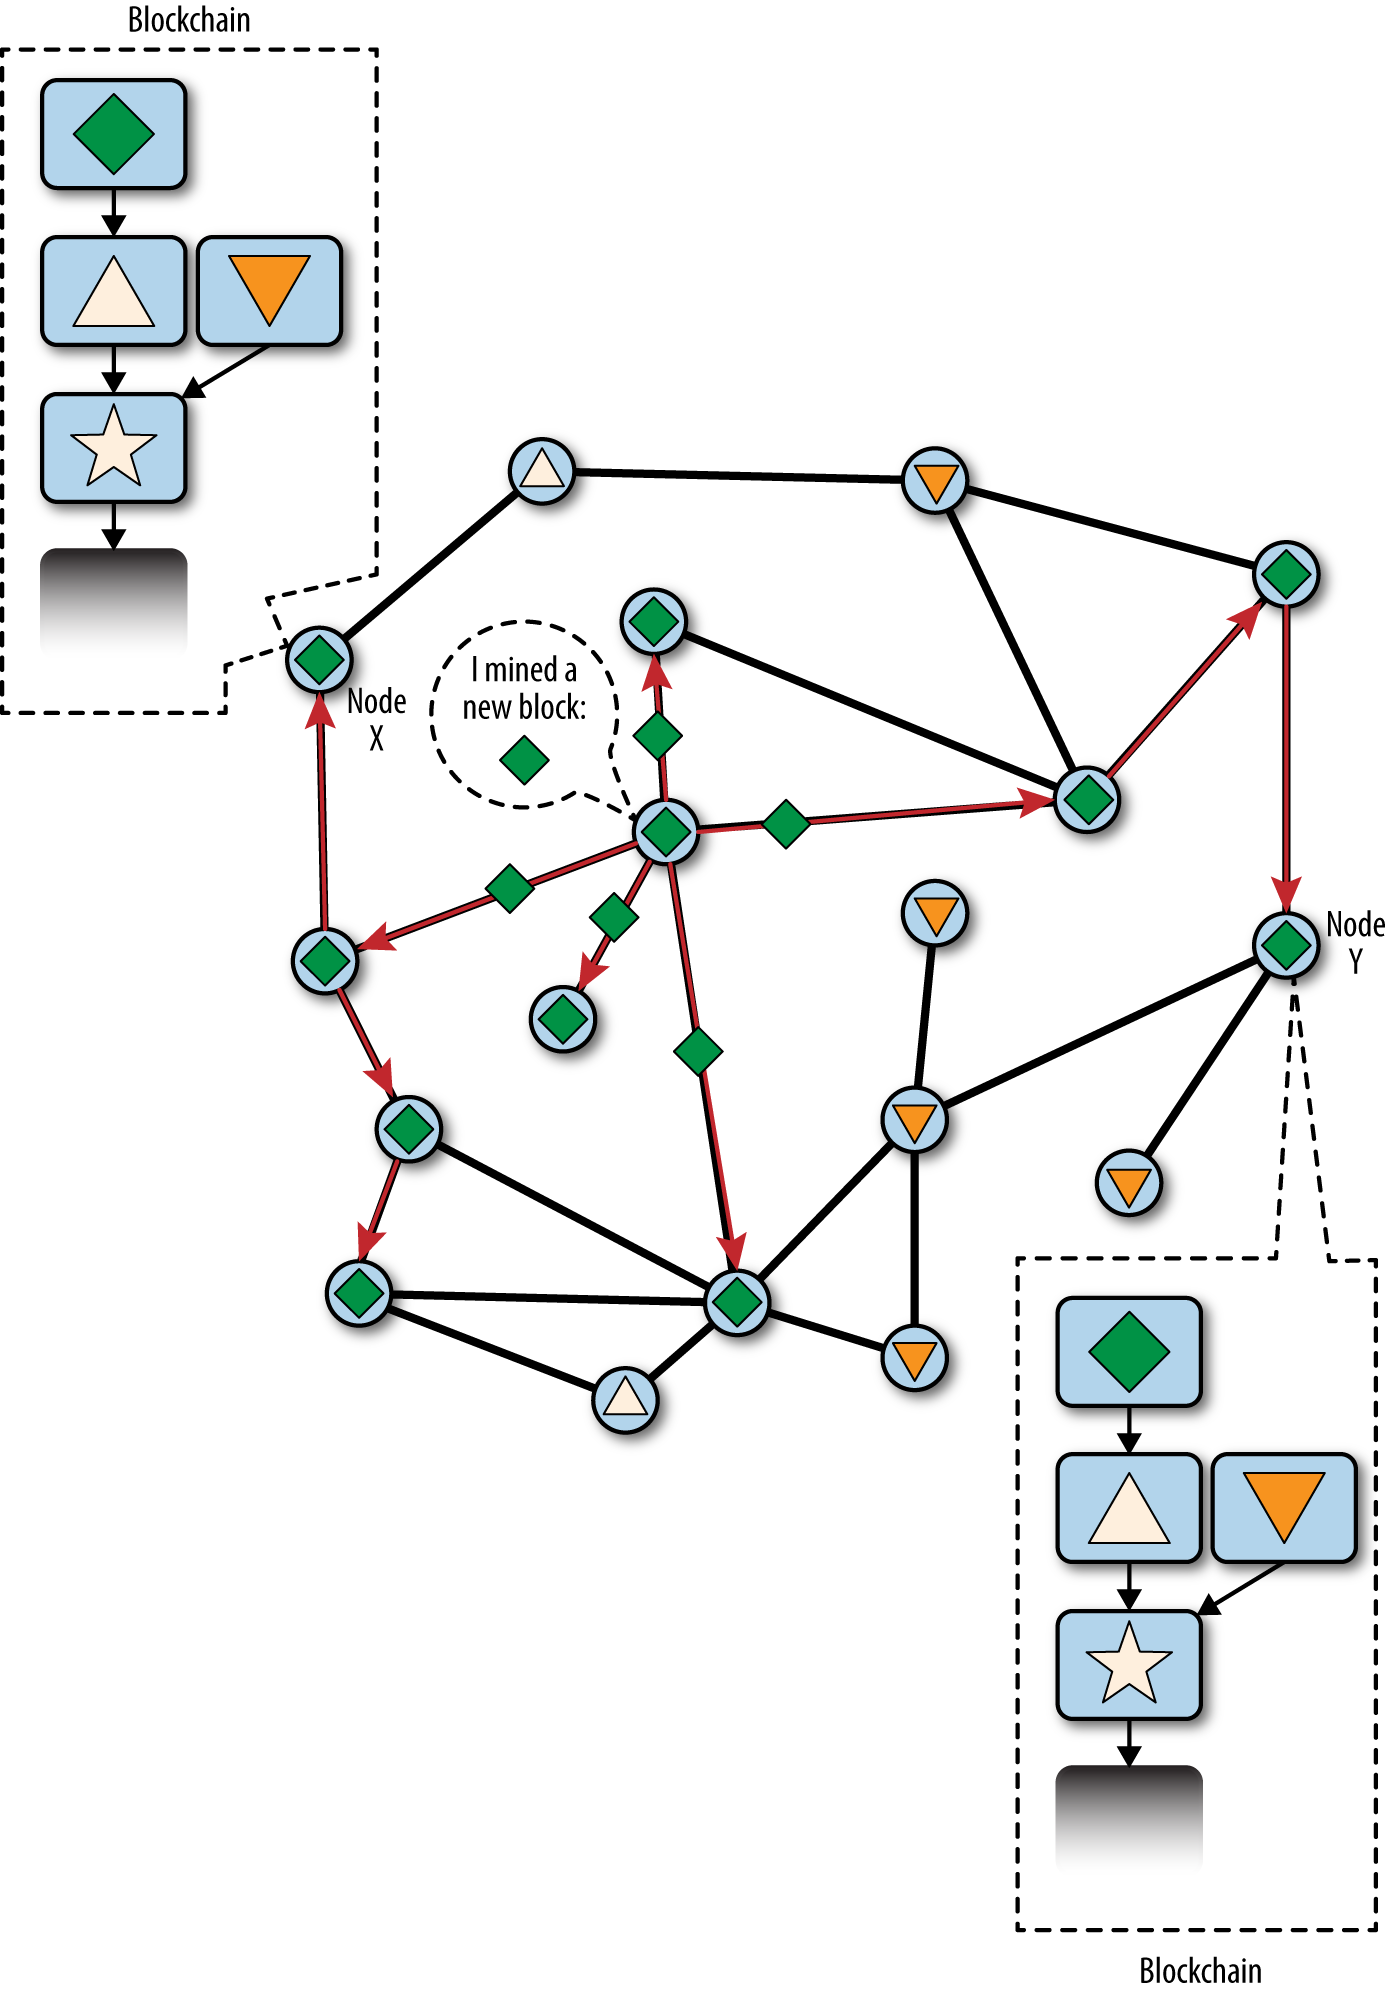
\includegraphics[scale=0.47,clip=false]{pictures/mbc2_1005.png}
  \end{center}

\end{frame}

\begin{frame}\frametitle{Fork: the network reconverges}

  \begin{center}
    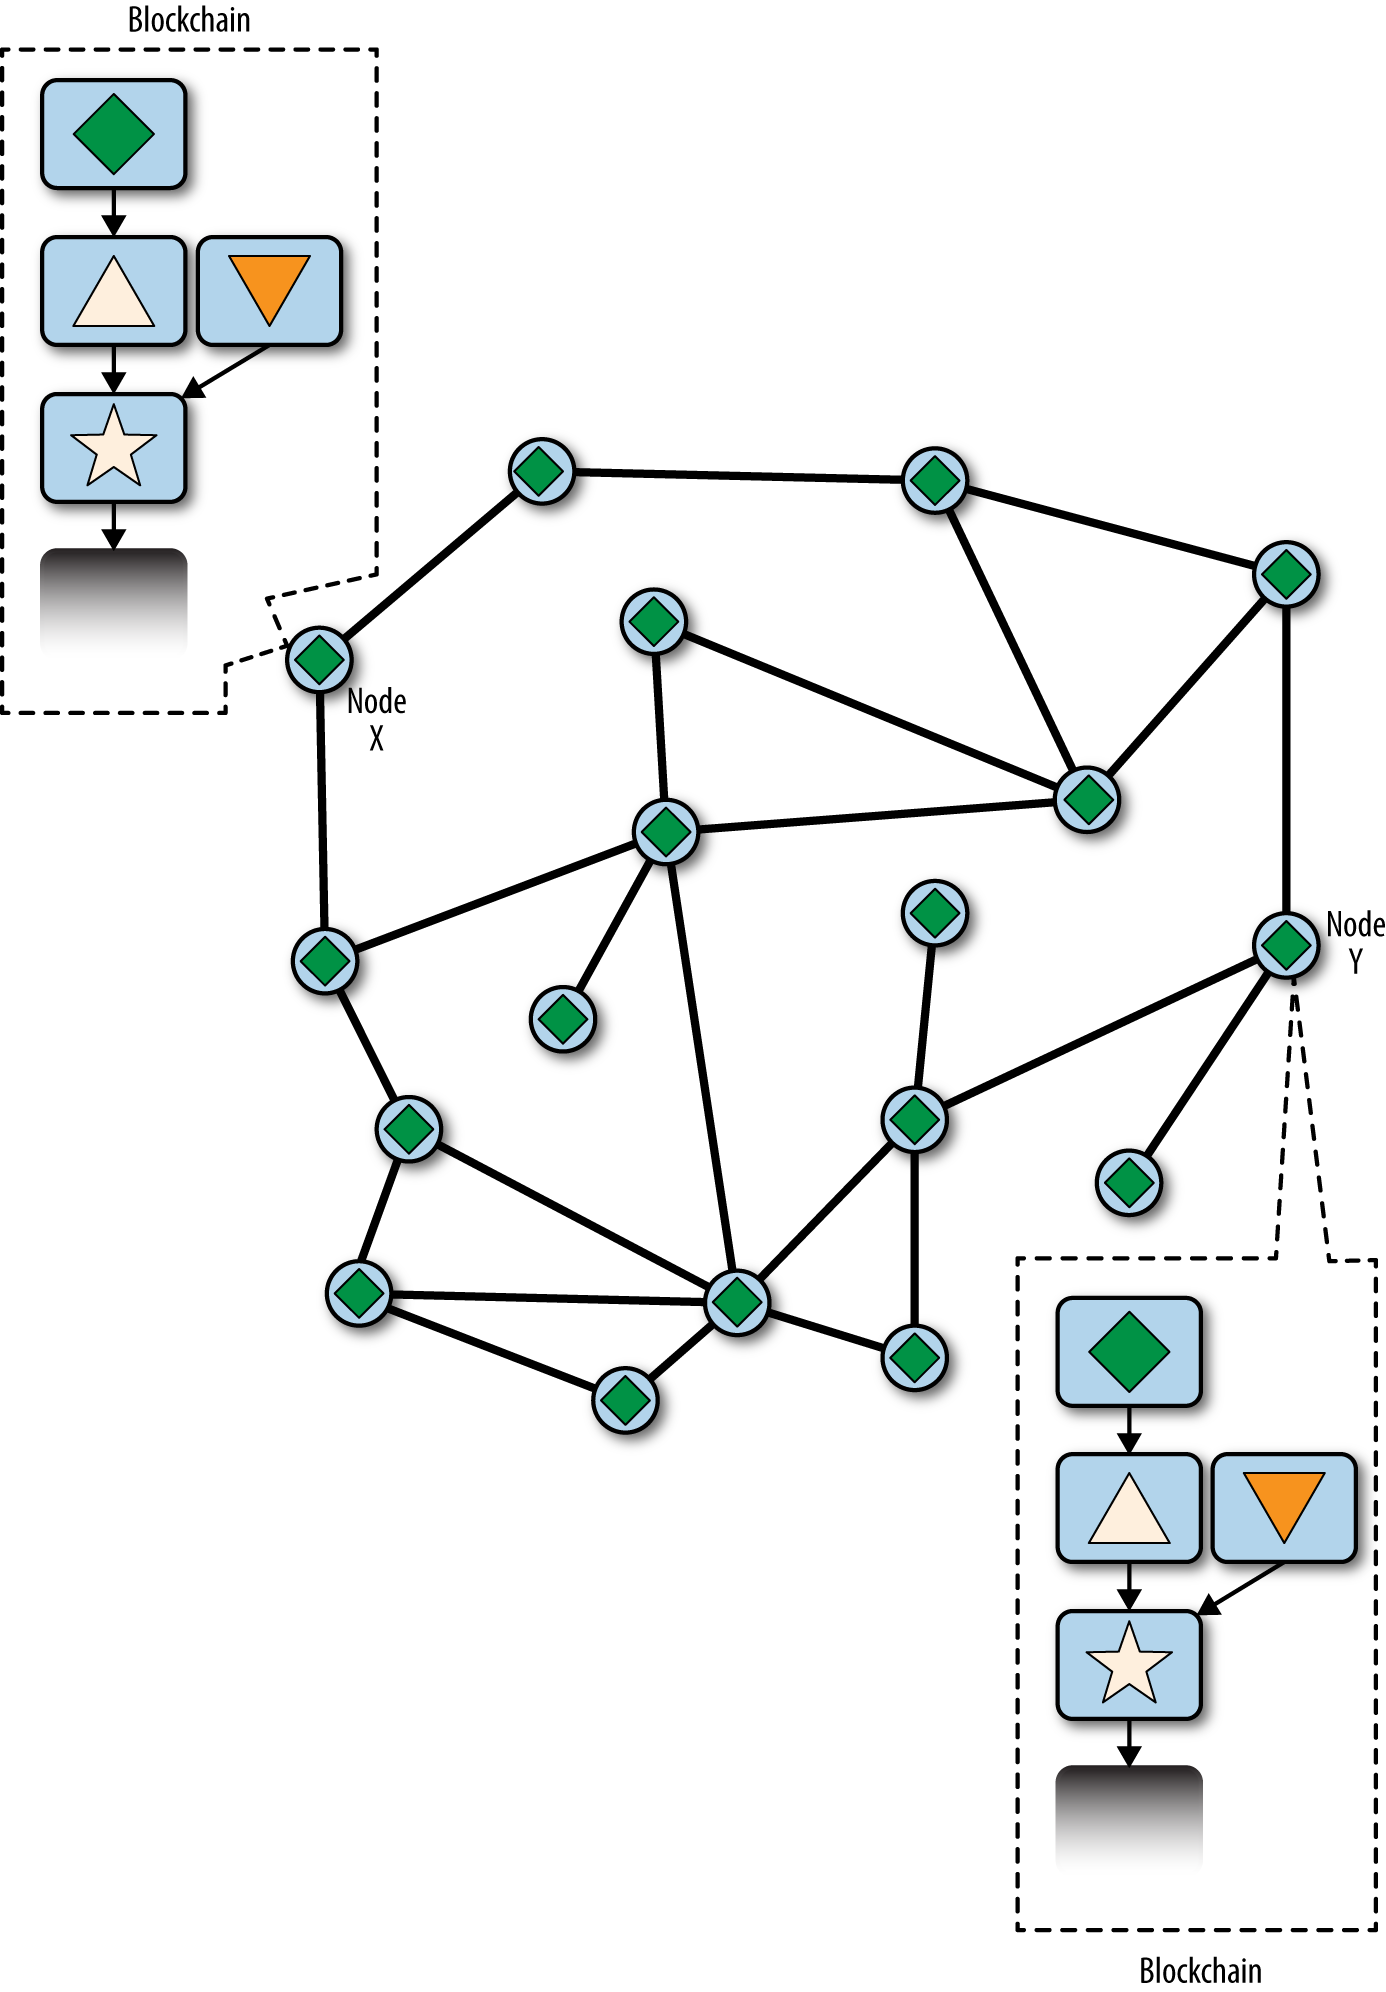
\includegraphics[scale=0.47,clip=false]{pictures/mbc2_1006.png}
  \end{center}

\end{frame}

\begin{frame}\frametitle{The magic behind PoW}

  \begin{greenbox}{}
    It makes expensive the production of new blocks, in time and cost (electricity)
    \begin{itemize}
    \item who produces invalid blocks sees its blocks rejected by peers and wastes resources
    \item a single node cannot drive the history, since it must fight against
      the hashing power of all other nodes together
    \item forks become unlikely, since the probability of two nodes finding a new block at the same time
      is small
    \end{itemize}
  \end{greenbox}

\end{frame}

\begin{frame}\frametitle{Difficulty over time}

  \begin{center}
    \includegraphics[width=\textwidth,clip=false]{pictures/difficulty.jpg}
  \end{center}

\end{frame}

\begin{frame}\frametitle{PoW costs electricity}

  \begin{greenbox}{2019}
    \begin{center}
      \includegraphics[scale=0.17,clip=false]{pictures/bitcoin-consumption.jpg}
      \includegraphics[scale=0.14,clip=false]{pictures/greta.jpg}
    \end{center}
  \end{greenbox}
    
\end{frame}

\begin{frame}\frametitle{Consensus attacks}

  \begin{greenbox}{Two main categories}
    \begin{enumerate}
    \item history change (for the topmost few blocks)
    \item denial-of-service (against specific transactions or accounts)
    \end{enumerate}
  \end{greenbox}

  \bigskip

  Possible if the attacker controls a large portion of the total hashing power

  \begin{center}
    \includegraphics[scale=0.17,clip=false]{pictures/51-percenters.jpg}
  \end{center}

\end{frame}

\begin{frame}\frametitle{Bitcoin has probabilistic finality}

  \begin{center}
    \includegraphics[width=\textwidth,clip=false]{pictures/finality.png}
  \end{center}

\end{frame}

\section{Ethereum (smart contracts)}

\section{Tendermint (BFT, proof of stake)}

\section{Takamaka + Hotmoka}

\end{document}
